% Options for packages loaded elsewhere
\PassOptionsToPackage{unicode}{hyperref}
\PassOptionsToPackage{hyphens}{url}
\PassOptionsToPackage{dvipsnames,svgnames,x11names}{xcolor}
%
\documentclass[
  10pt,
]{krantz}
\usepackage{amsmath,amssymb}
\usepackage{lmodern}
\usepackage{setspace}
\usepackage{iftex}
\ifPDFTeX
  \usepackage[T1]{fontenc}
  \usepackage[utf8]{inputenc}
  \usepackage{textcomp} % provide euro and other symbols
\else % if luatex or xetex
  \usepackage{unicode-math}
  \defaultfontfeatures{Scale=MatchLowercase}
  \defaultfontfeatures[\rmfamily]{Ligatures=TeX,Scale=1}
\fi
% Use upquote if available, for straight quotes in verbatim environments
\IfFileExists{upquote.sty}{\usepackage{upquote}}{}
\IfFileExists{microtype.sty}{% use microtype if available
  \usepackage[]{microtype}
  \UseMicrotypeSet[protrusion]{basicmath} % disable protrusion for tt fonts
}{}
\makeatletter
\@ifundefined{KOMAClassName}{% if non-KOMA class
  \IfFileExists{parskip.sty}{%
    \usepackage{parskip}
  }{% else
    \setlength{\parindent}{0pt}
    \setlength{\parskip}{6pt plus 2pt minus 1pt}}
}{% if KOMA class
  \KOMAoptions{parskip=half}}
\makeatother
\usepackage{xcolor}
\IfFileExists{xurl.sty}{\usepackage{xurl}}{} % add URL line breaks if available
\IfFileExists{bookmark.sty}{\usepackage{bookmark}}{\usepackage{hyperref}}
\hypersetup{
  pdftitle={Arts escèniques},
  pdfauthor={Ramiro Palau},
  colorlinks=true,
  linkcolor={Maroon},
  filecolor={Maroon},
  citecolor={Blue},
  urlcolor={Blue},
  pdfcreator={LaTeX via pandoc}}
\urlstyle{same} % disable monospaced font for URLs
\usepackage[left=3cm,right=3cm,top=0.85cm,bottom=3cm]{geometry}
\usepackage{color}
\usepackage{fancyvrb}
\newcommand{\VerbBar}{|}
\newcommand{\VERB}{\Verb[commandchars=\\\{\}]}
\DefineVerbatimEnvironment{Highlighting}{Verbatim}{commandchars=\\\{\}}
% Add ',fontsize=\small' for more characters per line
\usepackage{framed}
\definecolor{shadecolor}{RGB}{248,248,248}
\newenvironment{Shaded}{\begin{snugshade}}{\end{snugshade}}
\newcommand{\AlertTok}[1]{\textcolor[rgb]{0.94,0.16,0.16}{#1}}
\newcommand{\AnnotationTok}[1]{\textcolor[rgb]{0.56,0.35,0.01}{\textbf{\textit{#1}}}}
\newcommand{\AttributeTok}[1]{\textcolor[rgb]{0.77,0.63,0.00}{#1}}
\newcommand{\BaseNTok}[1]{\textcolor[rgb]{0.00,0.00,0.81}{#1}}
\newcommand{\BuiltInTok}[1]{#1}
\newcommand{\CharTok}[1]{\textcolor[rgb]{0.31,0.60,0.02}{#1}}
\newcommand{\CommentTok}[1]{\textcolor[rgb]{0.56,0.35,0.01}{\textit{#1}}}
\newcommand{\CommentVarTok}[1]{\textcolor[rgb]{0.56,0.35,0.01}{\textbf{\textit{#1}}}}
\newcommand{\ConstantTok}[1]{\textcolor[rgb]{0.00,0.00,0.00}{#1}}
\newcommand{\ControlFlowTok}[1]{\textcolor[rgb]{0.13,0.29,0.53}{\textbf{#1}}}
\newcommand{\DataTypeTok}[1]{\textcolor[rgb]{0.13,0.29,0.53}{#1}}
\newcommand{\DecValTok}[1]{\textcolor[rgb]{0.00,0.00,0.81}{#1}}
\newcommand{\DocumentationTok}[1]{\textcolor[rgb]{0.56,0.35,0.01}{\textbf{\textit{#1}}}}
\newcommand{\ErrorTok}[1]{\textcolor[rgb]{0.64,0.00,0.00}{\textbf{#1}}}
\newcommand{\ExtensionTok}[1]{#1}
\newcommand{\FloatTok}[1]{\textcolor[rgb]{0.00,0.00,0.81}{#1}}
\newcommand{\FunctionTok}[1]{\textcolor[rgb]{0.00,0.00,0.00}{#1}}
\newcommand{\ImportTok}[1]{#1}
\newcommand{\InformationTok}[1]{\textcolor[rgb]{0.56,0.35,0.01}{\textbf{\textit{#1}}}}
\newcommand{\KeywordTok}[1]{\textcolor[rgb]{0.13,0.29,0.53}{\textbf{#1}}}
\newcommand{\NormalTok}[1]{#1}
\newcommand{\OperatorTok}[1]{\textcolor[rgb]{0.81,0.36,0.00}{\textbf{#1}}}
\newcommand{\OtherTok}[1]{\textcolor[rgb]{0.56,0.35,0.01}{#1}}
\newcommand{\PreprocessorTok}[1]{\textcolor[rgb]{0.56,0.35,0.01}{\textit{#1}}}
\newcommand{\RegionMarkerTok}[1]{#1}
\newcommand{\SpecialCharTok}[1]{\textcolor[rgb]{0.00,0.00,0.00}{#1}}
\newcommand{\SpecialStringTok}[1]{\textcolor[rgb]{0.31,0.60,0.02}{#1}}
\newcommand{\StringTok}[1]{\textcolor[rgb]{0.31,0.60,0.02}{#1}}
\newcommand{\VariableTok}[1]{\textcolor[rgb]{0.00,0.00,0.00}{#1}}
\newcommand{\VerbatimStringTok}[1]{\textcolor[rgb]{0.31,0.60,0.02}{#1}}
\newcommand{\WarningTok}[1]{\textcolor[rgb]{0.56,0.35,0.01}{\textbf{\textit{#1}}}}
\usepackage{longtable,booktabs,array}
\usepackage{calc} % for calculating minipage widths
% Correct order of tables after \paragraph or \subparagraph
\usepackage{etoolbox}
\makeatletter
\patchcmd\longtable{\par}{\if@noskipsec\mbox{}\fi\par}{}{}
\makeatother
% Allow footnotes in longtable head/foot
\IfFileExists{footnotehyper.sty}{\usepackage{footnotehyper}}{\usepackage{footnote}}
\makesavenoteenv{longtable}
\usepackage{graphicx}
\makeatletter
\def\maxwidth{\ifdim\Gin@nat@width>\linewidth\linewidth\else\Gin@nat@width\fi}
\def\maxheight{\ifdim\Gin@nat@height>\textheight\textheight\else\Gin@nat@height\fi}
\makeatother
% Scale images if necessary, so that they will not overflow the page
% margins by default, and it is still possible to overwrite the defaults
% using explicit options in \includegraphics[width, height, ...]{}
\setkeys{Gin}{width=\maxwidth,height=\maxheight,keepaspectratio}
% Set default figure placement to htbp
\makeatletter
\def\fps@figure{htbp}
\makeatother
% Make links footnotes instead of hotlinks:
\DeclareRobustCommand{\href}[2]{#2\footnote{\url{#1}}}
\setlength{\emergencystretch}{3em} % prevent overfull lines
\providecommand{\tightlist}{%
  \setlength{\itemsep}{0pt}\setlength{\parskip}{0pt}}
\setcounter{secnumdepth}{5}
\usepackage{booktabs}
\usepackage[catalan]{babel}
\usepackage{longtable}

%no se  ue fan
%\usepackage[bf,singlelinecheck=off]{caption}
%\usepackage{Alegreya}
%\usepackage[scale=.7]{sourcecodepro}
%\usepackage{framed,color}

\usepackage[skins]{tcolorbox}

\definecolor{colortip}{RGB}{81,183,73}
\definecolor{colornote}{RGB}{119,136,153}
\definecolor{colorwarn}{RGB}{255,83,59}
\definecolor{colorinfo}{RGB}{92, 122, 234}
\definecolor{colorcuidao}{RGB}{251,188,5}

\tcbset{
  colbacktitle=white,
  enhanced,
  boxrule=9pt,
  sharp corners,
  attach boxed title to top left={yshift=-1.5mm, xshift=5mm},
  colback=white, 
  coltext=black, 
  leftrule=.3mm,
  rightrule=.3mm,
  bottomrule=.3mm,
  toprule=.3mm,
  boxsep=1pt, 
  arc=4pt 
}
\newtcolorbox{rmdcuidao}[1]{
  title=#1,
  drop small lifted shadow,
  coltitle=colorcuidao,
  colframe=colorcuidao, 
  colback=colorcuidao!5!
}
\newtcolorbox{rmdtip}[1]{
  title=#1,
  drop small lifted shadow,
  coltitle=colortip,
  colframe=colortip, 
  colback=colortip!5!
}

\newtcolorbox{rmdnote}[1]{
  title=#1,
  drop small lifted shadow,
  coltitle=colornote,
  colframe=colornote,
  colback=colornote!5!
}

\newtcolorbox{rmdwarn}[1]{
  title=#1,
  drop small lifted shadow,
  coltitle=colorwarn,
  colframe=colorwarn,
  colback=colorwarn!5!
}

\newtcolorbox{rmdinfo}{
  drop large lifted shadow,
  coltitle=colorinfo,
  colframe=colorinfo,
  colback=colorinfo!5!,
  capture=hbox
}

%\makeatother
% marca d'aigua
% https://github.com/callegar/LaTeX-draftwatermark
% https://github.com/callegar/LaTeX-everypage
% https://ctan.org/pkg/draftwatermark
% draftwatermark espacio inestable everypage
%\usepackage[angle=270,text=Espacio\ inestable,color=gray,pos={0.5in,3.5in},scale=0.25]{draftwatermark}
% draftwatermark 和 everypage 由同一个人维护,后者将停止维护
% https://github.com/CTeX-org/ctex-kit/issues/331
%\RecustomVerbatimEnvironment{Highlighting}{Verbatim}{commandchars=\\\{\}}
\ifLuaTeX
  \usepackage{selnolig}  % disable illegal ligatures
\fi
\usepackage[]{natbib}
\bibliographystyle{apalike}

\title{Arts escèniques}
\usepackage{etoolbox}
\makeatletter
\providecommand{\subtitle}[1]{% add subtitle to \maketitle
  \apptocmd{\@title}{\par {\large #1 \par}}{}{}
}
\makeatother
\subtitle{Projecte de pràctiques d'empresa del grau\\
F.P. ASISX\\
I.E. Maria Enriquez\\
\emph{Gandia 2022}}
\author{Ramiro Palau}
\date{2022-05-10}

\begin{document}
\maketitle

{
\hypersetup{linkcolor=}
\setcounter{tocdepth}{2}
\tableofcontents
}
\setstretch{1}
\hypertarget{about}{%
\chapter*{About}\label{about}}


Documentació dels projectes proposats a realitzar en el desenvolupament de les pràctiques realitzades en \textbf{Espacio Inestable}.

\hypertarget{usage}{%
\section*{Usage}\label{usage}}


Anirem detallant els diferents projectes que se suggereixen per a digitalitzar \emph{les arts escèniques}, amb una breu descripció de la seua posada en funcionament, requisits, pros i contres.

En cas afirmatiu s'aniria desenvolupant la manera d'implantar-lo, cost, i detallarem el seu funcionament i configuració.

La idea, es que aquest document siga una guia per mantenir els projectes elaborats o replicar-los en altres llocs, i anar actualitzant els recursos, com forme evolucione la tecnologia i necessitats de l'empresa.

\hypertarget{reproducciuxf3-en-luxednia}{%
\chapter{Reproducció en línia}\label{reproducciuxf3-en-luxednia}}

\emph{Implantació d'un sistema de reproducció en línia per a la sala}

Es vol posar un sistema de streaming per a la sala i les seues funcions, o per tindre una còpia de les obres per poder-les editar més tard.

\hypertarget{materials}{%
\section{Materials}\label{materials}}

\emph{Es requeriria}

\begin{enumerate}
\def\labelenumi{\arabic{enumi}.}
\item
  \textbf{Servidor}, podria ser un ordinador de sobretaula, es pot mirar el que es gasta ara per a la venda d'entrades, per veure si compleix els requisits mínims per als serveis que finalment es volen donar, o un servidor dedicat, on centralitzem tots els serveis. (Comentaré aquest cas en l'apartat servidor)
\item
  \textbf{Un servidor de disc}, que podria ser el servidor dels altres apartats per guardar una còpia de les diferents càmeres. Si hi ha pressupost, es faria un \href{https://ca.wikipedia.org/wiki/RAID}{RAID 5}.
\item
  \textbf{Càmeres ip} i millors \textbf{micròfons} que envien el so per la connexió de xarxa de la càmera.
\item
  \href{https://www.vadavo.com/blog/switch-poe-que-es-y-que-tipos-hay/}{\textbf{Switch}} \href{https://ca.wikipedia.org/wiki/Power_over_Ethernet}{\textbf{PoE}}, es podria posar una de 4 ports en l'escenari, per a facilitar l'escalat posterior del projecte que no són massa cars, i un switch (aquest no PoE) en les oficines per centralitzar la xarxa. Tirar cable entre ells i les càmeres. Reduint la distància del PoE a les càmeres ip.
\end{enumerate}

\begin{rmdtip}{Consell}
Examinat la distribució del teatre, el millor és fer una topologia senzilla de la xarxa, Posar un switch i el servidor, en el quarto de les llums que està centrat, seria un bon joc, i d'alli traure cables a la resta dels departaments.

\end{rmdtip}

\begin{enumerate}
\def\labelenumi{\arabic{enumi}.}
\setcounter{enumi}{4}
\item
  \textbf{Conte} en una plataforma de streaming de l'elecció de la sala, youtube, \href{https://www.twitch.tv/}{twitch}.
\item
  \textbf{Programa de streaming} (OBS, Livestream Studio, Wirecast, vMix, mimoLive o Tricaster) alternatives gratuïtes.
\item
  Un ordinador o portàtil que duga a terme les tasques de \textbf{producció}, podria ser un dels ordinadors de l'empresa que gasta per a disseny, s'utilitzaria en el moment de fer la producció en viu. Per a fer streaming d'una obra editada a posteriori, de les còpies fetes en el servidor de disc, no faria falta.
\end{enumerate}

\hypertarget{projecte-dinstillaciuxf3}{%
\section{Projecte d'instil·lació}\label{projecte-dinstillaciuxf3}}

Es faria fent tres xarxes diferents, una per al circuit d'imatge i so de les càmeres, altra per al wifi de la sala i la tercera per als equips d'administració. Per això, necessitem un switch en l'oficina que puga fer diverses xarxes virtuals, per tindre-les separades. (no volem que un espectador puga entrar en els ordinadors de l'oficina, o sature internet i done latència al streaming)

\hypertarget{pressupost}{%
\section{Pressupost}\label{pressupost}}

\hypertarget{software}{%
\section{Software}\label{software}}

Programes de streaming, OBS, Livestream Studio, Wirecast, mimoLive.

Es recomana per a començar OBS o Livestream, en cas que l'ordinador que farà de centre de producció siga un Mac, l'opció serà OBS.

\begin{longtable}[]{@{}
  >{\raggedright\arraybackslash}p{(\columnwidth - 2\tabcolsep) * \real{0.4742}}
  >{\raggedright\arraybackslash}p{(\columnwidth - 2\tabcolsep) * \real{0.5258}}@{}}
\caption{Programes}\tabularnewline
\toprule
\begin{minipage}[b]{\linewidth}\raggedright
\textbf{Programes}
\end{minipage} & \begin{minipage}[b]{\linewidth}\raggedright
\textbf{Desc}
\end{minipage} \\
\midrule
\endfirsthead
\toprule
\begin{minipage}[b]{\linewidth}\raggedright
\textbf{Programes}
\end{minipage} & \begin{minipage}[b]{\linewidth}\raggedright
\textbf{Desc}
\end{minipage} \\
\midrule
\endhead
\href{https://obsproject.com/}{OBS} & Programari gratis per a gravar video i streaming. \\
\href{https://streamlabs.com/}{Livestream Studio} & Per a Windows \\
\href{https://www.telestream.net/}{Wirecast} & De pagament. \\
\href{https://mimolive.com/}{MimoLive} & Pagament processional. \\
\bottomrule
\end{longtable}

\hypertarget{hardware-necessari}{%
\section{Hardware necessari}\label{hardware-necessari}}

\hypertarget{servidor}{%
\subsection{Servidor}\label{servidor}}

Es comenta que es pot reutilitzar l'ordinador que es te en venda d'entrades, es pot mirar a veure si compleix els requisits mínims requerits. En principi, no crec que faça falta un massa potent per al que volem posar.

En el servidor s'implementaran serveis de DNS, Servidor de fulles web, (controlador de domini, no crec que siga necessari, però es pot posar també, si volem controlar els recursos que tinga accés cada membre)

Es podia discutir si interessa un sistema de comunicacions intern, per poder comunicar mitjançant so, vídeo o xat entre el control i l'escenari. o volen passar informació en temps real als actors en l'escenari des de control. hi ha diverses opcions lliures, per exemple \href{https://meet.jit.si/}{Jitsi meet}, hauria de mirar-ho, ho he de provar varie vegades, i no he pogut fer-lo funcionar, es cosa d'insistir. Aço li donaria un poc mes de faena al servidor, però com no serien molts interlocutors, no crec que requerisca massa potencia.

Es podria posar també un sistema de \href{https://nextcloud.com/}{cloud} intern, que ja integra les videoconferències i moltes més coses per al treball en equip, però supose que amb un equip reduït, igual no val la pena, si soles es local, i la gent treballa des de casa la major part del temps. Es pot contractar un conte en línia, però ja s'està gastant el drive. Es pot fer una demo, i si interessa es deixa.

Sistema de correu intern, no li veig massa sentit, però es pot posar.

Al servidor de web, es pot instal·lar una còpia de WordPress, per si es vol experimentar com es veuen les coses abans de publicar-les. Es pot configurar perquè cada usuari de la sala tinga el seu directori per penjar les seues fulles.

Crec que seria interessant, per servir presentacions de les obres que es van a representar, si al final s'instal·la wifi en la sala, que tinguen una primera fulla al connectar, on es parle de l'obra que van a veure, de les pròximes que es representaran una fulla, o on es puga interactuar amb ells, passant qüestionaris, convidant-los a fer comentaris \ldots{} ( açò es intern i soles es pot realitzar amb la gent que es connecte al wifi)

En principi l'ordinador per fer el streaming, ha de tindre una targeta de vídeo mitjanament potent, no crec que siga el cas del servidor, aquest no requereix ni pantalla una vegada instal·lat, es gastaria algun altre disponible en la sala, en cas necessari, ho podíem fer també en aquest, però va augmentant el nivell de requisits mínims de potència.

\texttt{Si\ se\ m\textquotesingle{}ocorre\ alguna\ cosa\ més\ la\ posaré,\ o\ ja\ em\ digueu.}

\hypertarget{servidor-de-disc}{%
\subsection{Servidor de disc}\label{servidor-de-disc}}

Si es volen guardar les còpies de les càmeres, i la idea es no fer un streaming pur, més bé editar a posteriori les imatges, o tindre una còpia dels assajos per veure en què es pot millorar, es requeriria espai per fer aquestes còpies. Hi ha dues possibilitats.

\begin{itemize}
\item
  \href{https://en.wikipedia.org/wiki/Network-attached_storage}{NAS}, sistema de disc en xarxa, La millor opció.
\item
  Que la torre que gastem de servidor , faça de servidor de disc, on es pot implementar configurar RAID en diferents tipus de redundàncies, segons el nombre de discs durs que tinguem, i si ens interessa més la velocitat o la redundància.
\end{itemize}

\hypertarget{cuxe0meres-ip}{%
\subsection{Càmeres ip}\label{cuxe0meres-ip}}

Hi ha dos tipus de càmeres ip que ens vindrien bé, unes són del tipus \href{https://ca.wikipedia.org/wiki/C\%C3\%A0mera_PTZ}{PTZ} es poden controlar remotament, i altres que són fixes, més barates. Es podria fer una mix dels dos tipus, la frontal a l'escenari, podria fer fixa, i en algun lateral posar una amb moviment.

El projecte es pot implantar per fases, primer provar en una, i si dona resultat anar ampliant, segons necessitats.

Per les característiques dels espectacles, es requeriria càmeres amb bona lluminositat, bones lents, açò augmentara el pressupost, pero segons les capacitats es pot anar fent, i millorar si es considera que val la pena.

Les càmeres i el muntatge està pensat per poder ser fàcilment desmuntable i transportat en cas de tindre la necessitat de realitzar l'espectacle extern a la sala. O reutilitzar el material obsolet per aquest fi.

\texttt{Llista\ provisional\ de\ recerca\ de\ càmeres\ i\ marques.}

\begin{itemize}
\item
  \href{https://www.amazon.es/dp/B086X637W2?ref_=as_li_ss_tl\&language=en_US\&linkCode=gs2\&linkId=a19d43bd6c875dd9cde44b1b4f5a3776\&tag=getlockers0f8-21\&th=1}{camera en amazon zowietek}
\item
  \href{https://www.axis.com/en-us/products/axis-v59-series}{Axis}
\item
  \href{https://getlockers.com/best-ptz-camera-for-live-streaming/}{Getlockers}
\item
  \href{https://ptzoptics.com/sdi/}{Ptzoptics}
\end{itemize}

\hypertarget{el-compte-del-streaming}{%
\subsection{El compte del streaming}\label{el-compte-del-streaming}}

És traure un compte en alguna de les plataformes que existeixen, ja teniu un compte en youtube, es pot gastar eixa o traure en \href{https://www.twitch.tv/}{twitch}, a veure quina deixa configurar més la pàgina d'inici, es pot crear una nova on enllaçar els continguts, o integrar-los en les fulles de l'empresa.

\hypertarget{muntatge}{%
\section{Muntatge}\label{muntatge}}

Faré proves de tot açò i penjaré el resultat de com es fa.

\hypertarget{cuxe0meres}{%
\section{càmeres}\label{cuxe0meres}}

L'únic requisit és que totes les vostres càmeres IP, independentment del fabricant, siguen compatibles amb el protocol ONVIF o el flux RTSP/MJPEG.

Les millors aplicacions de visualització de càmeres IP per a dispositius Android

\textbf{monitor tinyCAM} El monitor tinyCam ve en dues versions, la gratuïta amb funcions limitades i la versió professional de pagament. El bàsic pot funcionar bé si busqueu alguna cosa senzilla. Utilitza el protocol ONVIF, la transmissió RTSP, etc., i pot transmetre en directe el canal de vídeo sense cap retard. La versió de pagament és d'uns 5 dòlars i és un pagament únic. Podeu utilitzar aquesta aplicació per veure la vista en directe de les vostres càmeres 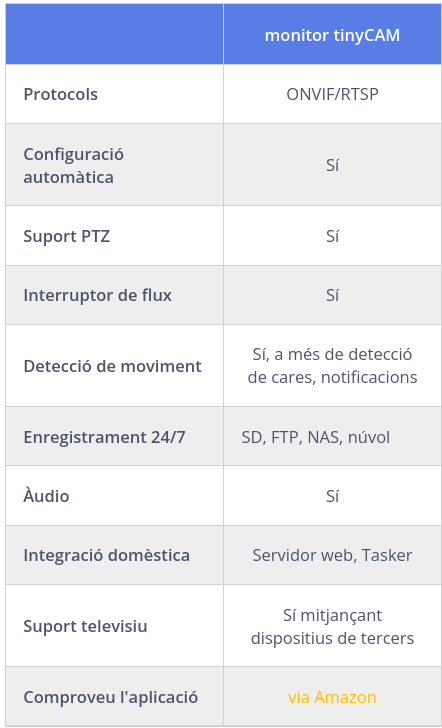
\includegraphics{imatges/tinycam.png}

\hypertarget{la-gravadora-nvr}{%
\section{La gravadora (NVR)}\label{la-gravadora-nvr}}

En un sistema de càmeres de seguretat IP, el NVR (Network Video Recorder) és central que gestiona i emmagatzema les imatges de vídeo. Totes les càmeres IP enviaran les seues dades a les gravadores des de les quals podeu visualitzar en directe o fer còpies de seguretat de les gravacions.

L'NVR està especialitzat a fer funcionar la càmera sense problemes, utilitzen diversos algorismes de compressió per gestionar i emmagatzemar el metratge de manera eficient. Depenent de la marca, podeu instal·lar 1-4 peces d'un disc dur a l'NVR. La qualitat de la imatge dels vídeos depén de la càmera (no de l'NVR), com més alta siga la resolució i més clara siga la imatge. Tots els sistemes de càmeres enumerats en aquesta guia ofereixen imatges d'alta resolució (4MP o més).

\href{https://www.amazon.es/dp/B07RYBHWZM/ref=as_li_tl?ie=UTF8\&linkCode=gs2\&linkId=5ffd9566b7959f94208952ac3587cf3e\&creativeASIN=B07RYBHWZM\&tag=rhp15904-21\&creative=9325\&camp=1789}{camera amcrestultra hd 4k} Amcrest UltraHD 4K (8MP) Càmera PoE de Seguridad IP para Exteriores, 3840 x 2160, 164 pies de visión Nocturna, Lente de 2,8 mm, IP67 Resistente a la Intemperie, grabación MicroSD \textbf{239,68€} \textbf{Cuenta con una capacidad mejorada de poca luz utilizando el último sensor de imagen IMX274 Sony Starvis y el chipset S3LM Ambarella.} 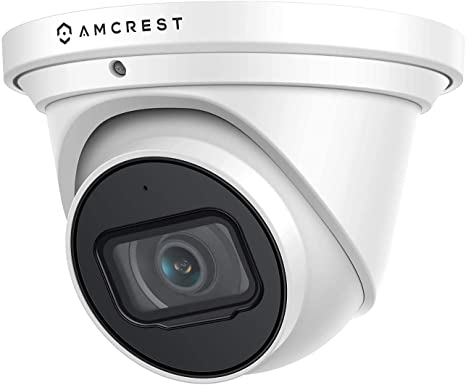
\includegraphics{imatges/amcrest.jpg}

CCTV AND NVR SOLUTION INSTALLATION GUIDE FOR UBUNTU 20.04 LINUX! \href{https://hendgrow.com/2020/12/30/33-cctv-and-nvr-solution-installation-guide-for-ubuntu-20-04-linux/}{install}

\href{https://hendgrow.com/ugs/HendGrow_CCTV_Text_Guide.txt}{Location of text walk through:}

\begin{verbatim}
Guide Start

Download the install script
$ sudo wget https://gitlab.com/Shinobi-Systems/Shinobi-Installer/raw/master/shinobi-install.sh
$ sudo chmod 777 shinobi-install.sh
$ sudo ./shinobi-install.sh

Installtion prompt responses 
---------------------------------------------
Install the Development branch?
(y)es or (N)o? Default : No
->No
---------------------------------------------
========
Select your OS
If your OS is not on the list please refer to the docs.
========
1. Ubuntu - Fast and Touchless
2. Ubuntu - Advanced
3. CentOS
4. CentOS - Quick Install
5. MacOS
6. FreeBSD
7. OpenSUSE
========
-> 1
---------------------------------------------
Shinobi - Do you want to temporarily disable IPv6?
Sometimes IPv6 causes Ubuntu package updates to fail. Only do this if your machine doesn't rely on IPv6.
(y)es or (N)o
-> Y
---------------------------------------------
=====================================
||=====   Install Completed   =====||
=====================================
|| Login with the Superuser and create a new user!!
||===================================
|| Open http://172.16.195.4:8080/super in your web browser.
||===================================
|| Default Superuser : admin@shinobi.video
|| Default Password : admin
=====================================
=====================================
-----------------------------------------------

Once you have created your admin user under the /super url navigate to http://YOUR_RPI_IP_ADDRESS and login with the credentials you created.
\end{verbatim}

• 720p outdoor analog and IP PoE PTZ security camera price would be \$70-\$200. • 1080p PoE PTZ IP camera price is typically \$130-\$400. • 4MP (1440p) \& 5MP outdoor PoE PTZ IP camera price is \$200-\$600. • The 4K Ultra HD outdoor PTZ security camera price range is \$1000-\$3000. • The price of outdoor PoE PTZ dome cameras with auto motion tracking is \$300-\$700.

\hypertarget{zonaminder}{%
\section{\texorpdfstring{\href{https://zoneminder.com/downloads/}{zonaminder}}{zonaminder}}\label{zonaminder}}

\href{https://community.home-assistant.io/t/my-opinion-zoneminder-vs-motioneye-vs-shinobi/316831}{resenya} \href{https://www.turnkeylinux.org/zoneminder}{VM zonaminder} {[}docu{]}/\url{https://zoneminder.readthedocs.io/en/latest/userguide/definemonitor.html}

Track Motion Aquesta i les quatre opcions següents s'utilitzen amb la funció de moviment experimental. Això només funcionarà si la vostra càmera admet modes de moviment mapejat en què un punt d'una imatge es pot assignar a una comanda de control. Això és generalment més comú a les càmeres de xarxa, però es pot replicar fins a cert punt en altres càmeres que admeten modes de moviment relatiu. Consulteu la secció Control de la càmera per obtenir més detalls. Marqueu aquesta casella per activar el seguiment de moviment.

\textbf{estimacio de memoria que necesita} \href{https://zoneminder.readthedocs.io/en/latest/faq.html}{ref}

Min Bits of Memory = 20\% overhead * (image-width\emph{image-height}image buffer size\emph{target color space}number of cameras) image-width i image-height són l'amplada i l'alçada de les imatges per a les quals està configurada la càmera (en el meu cas, 1280x960). Aquest valor es troba a la pestanya Font de cada monitor La mida de la memòria intermèdia és el nombre d'imatges que ZM conservarà a la memòria (ZM l'utilitza per assegurar-se que té imatges prèvies i posteriors abans de detectar una alarma; molt útil perquè quan es detecta una alarma, el motiu de l'alarma pot ser sortir de la vista i un buffer és realment útil per a això, inclòs per analitzar estadístiques/puntuació). Aquest valor es troba a la pestanya de memòria intermèdia de cada monitor L'espai de color objectiu és la profunditat de color: 8 bits, 24 bits o 32 bits. Torna a estar a la pestanya font de cada monitor

La sobrecàrrega del 20\% a la part superior del càlcul per tenir en compte les despeses generals d'imatge/stream (aquesta és una estimació)

El desglossament matemàtic de 4 càmeres amb captura de 1280 x 960, memòria intermèdia de 50 fotogrames, espai de color de 24 bits:

\begin{verbatim}
1280*960 = 1,228,800 (bytes)
1,228,800 * (3 bytes for 24 bit) = 3,686,400 (bytes)
3,686,400 * 50 = 184,320,000 (bytes)
184,320,000 * 4 = 737,280,000 (bytes)
737,280,000 / 1024 = 720,000 (Kilobytes)
720,000 / 1024 = 703.125 (Megabytes)
703.125 / 1024 = 0.686 (Gigabytes)
\end{verbatim}

Uns 700 MB de memòria.

Així que si teniu 2 GB de memòria, hauríeu d'estar tot a punt. Dret? No, realment:

\begin{itemize}
\tightlist
\item
  Aquesta és només la memòria base necessària per capturar els fluxos. Recordeu que ZM sempre està capturant fluxos, independentment de si realment esteu gravant o no, per assegurar-vos que el seu buffer d'anell d'imatge hi hagi amb imatges prèvies quan s'activa una alarma.
\item
  També heu de tenir en compte altres processos no relacionats amb ZM que s'executen a la vostra caixa
\item
  També heu de tenir en compte altres processos ZM; per exemple, em vaig adonar que el dimoni d'auditoria ocupa una bona quantitat de memòria quan s'executa, les actualitzacions de la base de dades també ocupen memòria.
\item
  Si utilitzeu la codificació H264, també emmagatzema molts fotogrames a la memòria.
\end{itemize}

Per tant, una bona regla general és assegurar-vos que teniu el doble de memòria que el càlcul anterior (i si feu servir el servidor ZM per a altres propòsits, tingueu en compte aquests requisits de memòria també).

Recordeu també que per defecte ZM només utilitza el 50\% de la vostra memòria disponible tret que la canvieu

Com a resultat, ZM utilitza memòria mapejada i, de manera predeterminada, el 50\% de la vostra memòria física és el que arribarà. Quan arribeu a aquest límit, ZM es descompon amb diversos errors.

Una bona manera de saber quanta memòria s'assigna a ZM per al seu funcionament és fer adf -h

\textbf{cpu}

Els diferents elements de ZoneMinder poden estar implicats en una activitat força intensa, especialment mentre s'analitzen imatges per veure'n el moviment. Tanmateix, en general, això no hauria d'aclaparar la vostra màquina tret que sigui molt antiga o amb poca potència.

\begin{itemize}
\tightlist
\item
  unció d'execució. Òbviament, l'execució en els modes Record o Mocord o en Modect amb molts esdeveniments genera molta activitat de base de dades i fitxers i, per tant, augmentarà la CPU i la càrrega.
\item
  *Zones de detecció predeterminades bàsiques. Per defecte, quan s'afegeix una càmera, s'afegeix una zona de detecció que cobreix tota la imatge amb un conjunt de paràmetres per defecte. Si la vostra càmera cobreix una vista en la qual és poc probable que diverses regions generin una alarma vàlida (és a dir, el cel), experimentaria amb la reducció de la mida de les zones o afegint zones inactives per esborrar àrees que no voleu controlar.
\item
  Per exemple, si tinc un dimoni ``zma'' \hspace{0pt}\hspace{0pt}en execució per a un monitor que està capturant una imatge. He comentat l'anàlisi real, així que tot el que fa és combinar la imatge amb l'anterior. En mode de color, això triga \textasciitilde{} 11 mil·lisegons per fotograma al meu sistema i la càmera està capturant a \textasciitilde{} 10 fps. Si utilitzeu `superior', s'informa que el procés fa servir el \textasciitilde5\% de la CPU i que està permanentment en estat R(un). En canviar al mode d'escala de grisos, la combinació triga \textasciitilde{} 4 ms (com és d'esperar, ja que és aproximadament un terç d'11), però la part superior informa que el procés és ara amb 0\% de CPU i permanentment en estat S (leep). Per tant, un canvi real d'ús de recursos de la CPU d'un factor de 3 provoca grans diferències en l'ús de la CPU informat.
\end{itemize}

\emph{CPU en camara ip}

En mode modect

Les càmeres IP requereixen un nivell addicional de processament a les targetes analògiques, ja que les imatges jpg o mjpeg s'han de descodificar abans d'analitzar-les. Això necessita grunyits. Si teniu moltes càmeres, necessiteu molts grunyits.

\emph{solucions} * Augmenta la memòria RAM. Si el vostre sistema ha d'utilitzar l'intercanvi de disc, afectarà Enormement el rendiment en totes les àrees. * Zoneminder també funciona molt bé amb diversos sistemes de processadors fora de la caixa (si SMP està habilitat al vostre nucli). La càrrega de diferents càmeres es distribueix entre els processadors. *

\textbf{Disc dur}

Com a guia ràpida, tinc 4 càmeres a 320x240 que emmagatzemen 1 fps excepte durant els esdeveniments d'alarma. Després d'1 setmana, s'han utilitzat 60 GB d'espai al volum on s'emmagatzemen els esdeveniments (/var/www/html/zm). \href{https://www.digitalrebellion.com/webapps/videocalc}{Calcul de espai}

\begin{verbatim}
Format  HDV 1080
Resolution  1440x1080
Frame rate  25
Video length 1 hours
Total space: 10.99 GB

Format  H.264 1080
Resolution  1920x1080
Frame rate  25
Video length 1 hours
Total space: 36.17 GB
\end{verbatim}

\textbf{Auto trackin}

zoneminder auto tracking zmtrack.pl

\textbf{xarxa} \emph{RTSP,} 1920 x 1080 at 60 FPS requires a bitrate or 12,288 Kb/s while the same resolution at 30 FPS only requires a bitrate of 8,192 Kb/s.

\emph{RTMP} \href{mailto:1920x1080@60fps}{\nolinkurl{1920x1080@60fps}} bitrate = 4,500 - 9,000 Kbps i-frame interval: 120 (2 seconds) CBR

\begin{verbatim}
1920x1080@30fps
bitrate = 3,000 - 6,000 Kbps
i-frame interval: 60 (2 seconds)
CBR
\end{verbatim}

Camera Settings for Low Light Performance Resolution: 1920x1080p 30fps Camera Aperture: small such as 1.8 Camera Shutter Speed: slow 1/120 Camera Focus: Manua

Low Light: Noise Reduction 2D Noise Reduction: Ideal for scenes with a lot of movement. 3D Noise Reduction: Ideal for static fields of view. Tip: Try using a combination of 2D \& 3D Noise Reduction for best results

\hypertarget{motioneye}{%
\section{Motioneye}\label{motioneye}}

\hypertarget{camare-ip-barates}{%
\section{camare ip barates}\label{camare-ip-barates}}

\href{https://www.amazon.com/-/es/autom\%C3\%A1tico-conferencia-omnidireccionales-seguimiento-transmisi\%C3\%B3n/dp/B09MVVVWS8/ref=sr_1_9?keywords=auto+tracking+ptz+camera\&qid=1652033445\&sr=8-9}{OBSBOT Tiny} PTZ Cámara web 4K, encuadre y enfoque automático, cámara de video conferencia 4K con micrófonos omnidireccionales duales, seguimiento automático con cardán de 2 ejes, HDR, 60 FPS, corrección de poca luz, transmisión US\$269.00 usb 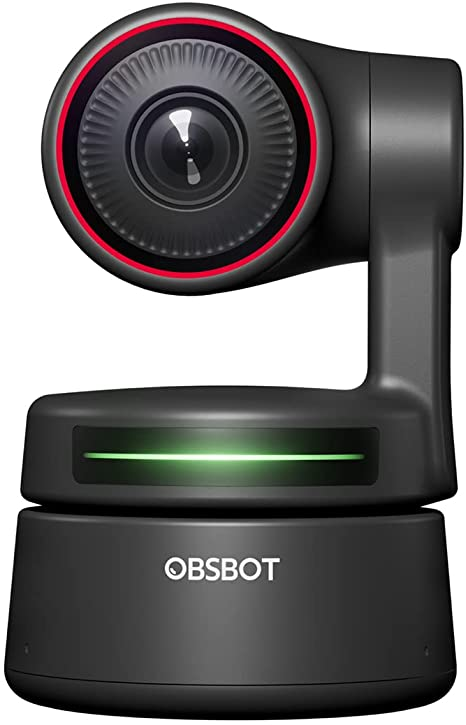
\includegraphics{imatges/obsbot.jpg}

Amcrest Cámara 4K POE AI Detección humano/vehículo, UltraHD 8MP Torreta de seguridad para exteriores POE Cámara IP, 3840x2160, gran angular, IP67 resistente a la intemperie, MicroSD, micrófono integrado, blanco (IP8M-T2669EW-AI) \href{https://www.amazon.com/-/es/Detecci\%C3\%B3n-exteriores-resistente-intemperie-IP8M-T2669EW-AI/dp/B08NXX27FR/ref=psdc_14241151_t2_B07RHQGS8V}{amcerest} US\$139.99 \href{https://m.media-amazon.com/images/I/71pf6+6KYIL.pdf}{espaecificacions} 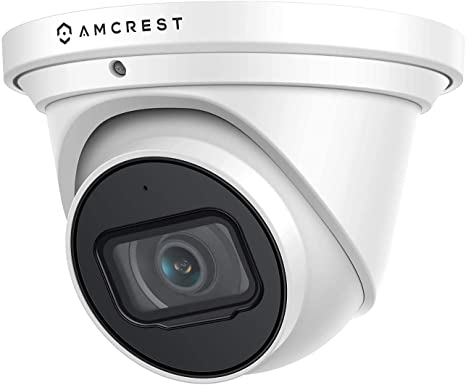
\includegraphics{imatges/amcrest.jpg}

Amcrest Cámara IP PoE con torreta AI de color nocturno con visión nocturna a todo color \href{https://www.amazon.com/-/es/seguridad-micr\%C3\%B3fono-integrado-detecci\%C3\%B3n-IP5M-T1273EW-AI/dp/B093X7W3GM/ref=sr_1_5?__mk_es_US=\%C3\%85M\%C3\%85\%C5\%BD\%C3\%95\%C3\%91\&crid=3OFUNOR4E9A7V\&keywords=poe+8mp+night+colour+security+camera\&qid=1652036679\&sprefix=camara+seguridad+poe+8+mp+color+nocturna\%2Caps\%2C192\&sr=8-5}{Amcrest Cámara IP PoE 5Mp} US\$89.99

Noise Reduction 3D DNR Storage FTP, Protocol IPv4, IPv6, HTTP, TCP, UDP, RTSP, TCP, RTMP, SMTP, FTP, DHCP, DDNS, UPnP, NTP

LA fixa \href{https://www.amazon.es/Amcrest-NightVision-resistente-intemperie-IP8M-2496EW-28MM/dp/B08SMPGF2L/ref=sr_1_1_sspa?__mk_es_ES=\%C3\%85M\%C3\%85\%C5\%BD\%C3\%95\%C3\%91\&crid=B563YL5W8NZG\&keywords=Amcrest\&qid=1652041726\&sprefix=amcrest\%2Caps\%2C93\&sr=8-1-spons\&psc=1\&spLa=ZW5jcnlwdGVkUXVhbGlmaWVyPUEzNU04RVpYSEg2MTNDJmVuY3J5cHRlZElkPUEwODgxOTQwRDUzMkNEVUg0QUVIJmVuY3J5cHRlZEFkSWQ9QTEwMTQxOTBBNzRSODlYRllZNk4md2lkZ2V0TmFtZT1zcF9hdGYmYWN0aW9uPWNsaWNrUmVkaXJlY3QmZG9Ob3RMb2dDbGljaz10cnVl}{Amcrest UltraHD 4K (8 MP) POE IP, cámara exterior, 3840 x 2160, 131 pies NightVision} 129,99€ \href{https://amcrest.com/downloadable/download/attachment/id/22371/}{especificacions}

\textbf{NightColor} La tecnologia d'avantguarda NightColor us permet obtenir una imatge nítida fins i tot quan és fosc. Aquesta càmera té 2 LED blancs que transmeten els seus raigs infrarojos en una freqüència imperceptible a l'ull humà. Les llums blanques emeten brillants que ofereixen una increïble gamma de NightColor de 66 peus. Amb aquesta potent funció, podeu obtenir una consciència total sobre allò que no s'havia vist anteriorment i fer-ho d'una manera indetectable.

\textbf{cameraes amb nightvolor} \href{https://www.amazon.es/Exteriores-Seguridad-vigilancia-detecci\%C3\%B3n-humanoide/dp/B09CMRTXCH/ref=sr_1_5?__mk_es_ES=\%C3\%85M\%C3\%85\%C5\%BD\%C3\%95\%C3\%91\&crid=1HGWT0B8AQ04L\&keywords=ptz+Visi\%C3\%B3n+Nocturna+a+Color+poe\&qid=1652043379\&s=tools\&sprefix=ptz+visi\%C3\%B3n+nocturna+a+color+poe\%2Cdiy\%2C95\&sr=1-5}{barata}

\href{https://www.amazon.es/Reolink-Seguridad-Seguimiento-Autom\%C3\%A1tico-Outdoor-V3/dp/B099F2LGSB/ref=sr_1_9?__mk_es_ES=\%C3\%85M\%C3\%85\%C5\%BD\%C3\%95\%C3\%91\&crid=1HGWT0B8AQ04L\&keywords=ptz+Visi\%C3\%B3n+Nocturna+a+Color+poe\&qid=1652043379\&s=tools\&sprefix=ptz+visi\%C3\%B3n+nocturna+a+color+poe\%2Cdiy\%2C95\&sr=1-9}{Reolink 5MP PTZ Cámara} 139,99€

\href{https://www.amazon.es/Reolink-Vigilancia-Bidireccional-Impermeable-RLC-812A/dp/B096K1P2RK/ref=sr_1_10?__mk_es_ES=\%C3\%85M\%C3\%85\%C5\%BD\%C3\%95\%C3\%91\&crid=1HGWT0B8AQ04L\&keywords=ptz+Visi\%C3\%B3n+Nocturna+a+Color+poe\&qid=1652043379\&s=tools\&sprefix=ptz+visi\%C3\%B3n+nocturna+a+color+poe\%2Cdiy\%2C95\&sr=1-10}{fixa reolink 4K} 94,99€

\hypertarget{implantaciuxf3-dentorn-git}{%
\chapter{Implantació d'entorn Git}\label{implantaciuxf3-dentorn-git}}

Explorar la forma d'integrar el concepte git en les arts escèniques. Explorar els avantatges del seguiment de versions, i el procés col·laboratiu per a l'elaboració de publicacions o la creació d'obres de teatre,

\hypertarget{implantaciuxf3-del-sistema-collaboratiu-en-el-desenvolupament-dobres-de-teatre.}{%
\section{Implantació del sistema col·laboratiu en el desenvolupament d'obres de teatre.}\label{implantaciuxf3-del-sistema-collaboratiu-en-el-desenvolupament-dobres-de-teatre.}}

\begin{itemize}
\tightlist
\item
  Es pot realitzar mitjançant la creació d'un compte en una de les plataformes Git que hi ha en internet,
\item
  Configurant un servidor git en el mateix centre de treball

  \begin{itemize}
  \tightlist
  \item
    Git i un servidor web, aquesta opció es per a gastar l'entorn git en consola, no es recomana per a l'empresa.
  \item
    Un entorn web, he fet proves en GitLab i Gitea, i el final crec que la millor opció és la de Gitea pel reduït gaste de recursos que fa i la facilitat d'ús.
  \item
    Es pot mirar d'enllaçar el repositori git en el conte de drive que té l'empresa, per fer un repositori privat per als membres.
  \end{itemize}
\end{itemize}

\hypertarget{beneficis-de-la-seua-implantaciuxf3}{%
\section{Beneficis de la seua implantació}\label{beneficis-de-la-seua-implantaciuxf3}}

Els beneficis són els mateixos que per a la creació de projectes informàtics, però que son poc utilitzat en el món de les lletres. \emph{Possibilitat de crear obres col·laboratives.}

\begin{itemize}
\tightlist
\item
  El guardat de les diferents versions segons va desenvolupant-se el projecte, i poder tornar en el temps si alguna cosa no va bé.
\item
  Bifurcar camins d'exploració en la creació literària.
\end{itemize}

\hypertarget{mode-de-funcionament}{%
\section{Mode de funcionament}\label{mode-de-funcionament}}

\hypertarget{breu-tutorial-per-al-funcionament}{%
\subsection{Breu tutorial per al funcionament}\label{breu-tutorial-per-al-funcionament}}

\hypertarget{installaciuxf3-dun-repositori-en-el-centre}{%
\section{Instal·lació d'un repositori en el centre}\label{installaciuxf3-dun-repositori-en-el-centre}}

Procés d'instal·lació d'un repositori de git

\begin{itemize}
\item
  Git i Apache \texttt{buscar\ la\ fulla\ on\ ho\ explica}
\item
  Instal·lació de \href{https://docs.gitea.io/en-us/}{gitea} , o bé directament, o per una imatge Docker
\item
  Servir el \href{https://www.permikkelsen.dk/how-to-host-your-git-repository-on-onedrive.html}{git} en un espai onedrive, pareix que és per consola, mirar algun client de git desktop que facilita les coses.
\end{itemize}

\hypertarget{possible-implantaciuxf3-en-el-repositori-en-internet}{%
\section{Possible implantació en el repositori en internet}\label{possible-implantaciuxf3-en-el-repositori-en-internet}}

El més fàcil seria traure un compte en una de les plataformes que hi ha en internet, el problema és el recel que tinga l'empresa pel tema de privacitat. Aquestes plataformes tenen l'opció de crear repositoris privats, on soles es pot connectar al que convideu.

\hypertarget{explorar-obsidian}{%
\section{\texorpdfstring{Explorar \href{https://obsidian.md/}{Obsidian}}{Explorar Obsidian}}\label{explorar-obsidian}}

Obsidian és un editor de notes en funcions de seguiment git, per veure diff i altres funcions. Prou interessant, o com a alternativa \href{https://www.zettlr.com/}{Zettlr}, dona error en posar diccionaris.\\
I implantació d'un servidor de \href{https://github.com/Erikvl87/docker-languagetool}{Languagetool}

\hypertarget{explorar-wikimedia-per-a-la-realitzaciuxf3-descriptura-collaborativa}{%
\section{Explorar Wikimedia per a la realització d'escriptura col·laborativa}\label{explorar-wikimedia-per-a-la-realitzaciuxf3-descriptura-collaborativa}}

L'escriptura col·laborativa mitjançant ferramentes de xarxa, com la Wikipedia, on és possible discutir els convits proposats, obrir discussions sobre el text analitzat. Es pot explorar el concepte de \href{https://es.wikipedia.org/wiki/Narrativa_hipertextual}{Narrativa hipertextual} fent servir aquesta ferramenta.

\hypertarget{migraciuxf3-de-les-fulles-web-a-hugo}{%
\chapter{Migració de les fulles web a Hugo}\label{migraciuxf3-de-les-fulles-web-a-hugo}}

\texttt{En\ principi\ descartat}

\hypertarget{avantatges-de-la-migraciuxf3}{%
\section{Avantatges de la migració}\label{avantatges-de-la-migraciuxf3}}

\emph{Hugo és un framework per a construir fulles estàtiques}

La fulla web de l'empresa està implementada en WordPress,Hugo és una alternativa per la realització del projecte d'aquesta fulla, on el seu manteniment i implementació és molt més senzilla. Hugo és un framework on una vegada configurat el tema de la fulla, els autors de les publicacions, soles han de penjar un document de text, en format Markdown perquè aquests nou posts es publique, l'organització en carpetes i mitjançant tags ens facilita molt l'administració del lloc, a més de la seua seguretat, ja que soles compartim fulles estètiques, sense fer ús de bases de dades, reduint considerablement el seu manteniment.

\hypertarget{mode-dimplementar-la-migraciuxf3}{%
\section{Mode d'implementar la migració}\label{mode-dimplementar-la-migraciuxf3}}

Una vegada que l'empresa passe la còpia de seguretat de les fulles WordPress, hi ha una forma de passar els posts a Markdown.

Ordenant en diferents carpetes, per contingut temàtic i autors, on cada autor o secció te la seua carpeta on colgar els nous posts, en fitxer de text \emph{md} i les imatges que vulga que apareguen.

\hypertarget{conversiuxf3-dels-posts-de-wordpress-a-md}{%
\subsection{Conversió dels posts de WordPress a md}\label{conversiuxf3-dels-posts-de-wordpress-a-md}}

Possibles solucions per al procés

\begin{itemize}
\tightlist
\item
  \href{https://kevq.uk/how-to-convert-wordpress-to-markdown/}{How To Convert WordPress To Markdown}
\item
  \href{https://swizec.com/blog/how-to-export-a-large-wordpress-site-to-markdown/}{How to export a large Wordpress site to Markdown}
\item
  \href{https://prefetch.net/blog/2017/11/24/exporting-wordpress-posts-to-markdown/}{Exporting Wordpress Posts To Markdown}
\end{itemize}

\emph{Quan estiguem en el cas estudiarem en més profunditat la manera de fer-ho}

Estic mirant per a fer una xicoteta demostració de les característiques d'Hugo, per fer una posada en comú de com funciona, i si és factible la seua migració.

Una altra possibilitat de la seua implantació, és si es realitza la instal·lació d'una zona wifi en el pati de butaques, a l'hora de donar els paràmetres de la xarxa (nom de xarxa i contrasenya), que es faria en un codi \href{https://www.qr-code-generator.com/solutions/wifi-qr-code/}{QR} \emph{(alguna cosa pareguda açò, ja ho desenvoluparé un poc mes en l'apartat wifi)}, es pot passar una direcció d'entrada automàtica a una fulla web, que estaria en el servidor de la xarxa local, on es pot passar informació de l'obra que és representar, o realitzar interacció amb el públic, en temps real.

\hypertarget{possibles-interaccions-amb-el-puxfablic}{%
\subsubsection{Possibles interaccions amb el públic}\label{possibles-interaccions-amb-el-puxfablic}}

Les fulles del servidor intern per al públic, recomane que es facen amb Hugo, ho deixaré preparat perquè siga molt fàcil la creació de fulles noves. On soles s'ha de colgar un fitxer de text en un directori determinat\ldots{} bo, i compilar la fulla, però ja deixaré un script que ho faça, miraré la forma de fer-ho soles, integració continuada crec que es diu. Es pot fer en WordPress si vos és més fàcil, és parlar-ho i provar.

\begin{itemize}
\item
  Preàmbul de l'obra que es va a representar, perquè el públic s'informe o posar en context de què van a veure, uns minuts abans que comence.
\item
  Es pot dur a terme una web app de xat per a conferències, el públic puga colgar allí les seues preguntes, i des de la taula, poder seleccionar les més interessants, o la persona a la qual es donara veu.
\item
  Fer obres interactives amb el públic, on aquest puga fer votacions, mitjançant el seu mòbil, i d'aquesta forma poder canviar el desenllaç de l'obra en temps real.
\end{itemize}

En definitiva, si es configura una xarxa en la sala, poder traure tot el rendiment possible, ja que en l'actualitat tot el món té un mòbil damunt.

\hypertarget{organitzaciuxf3-dels-diferents-apartats-de-les-fulles}{%
\section{Organització dels diferents apartats de les fulles}\label{organitzaciuxf3-dels-diferents-apartats-de-les-fulles}}

\hypertarget{alternativa-merege-wordpress}{%
\section{Alternativa, merege WordPress}\label{alternativa-merege-wordpress}}

En cas contrari, es miraria la forma de combinar els 5 WordPress en un sol, fer \href{https://wpmudev.com/blog/merging-wordpress-sites/}{merge wordpress} \texttt{mirar\ que\ més\ alternatives\ hi\ ha.}

\hypertarget{implantaciuxf3-de-projectes-exelearning}{%
\chapter{Implantació de projectes Exelearning}\label{implantaciuxf3-de-projectes-exelearning}}

\href{https://exelearning.net/ca}{Exelearning} és una eina d'autor de codi obert per ajudar als docents en la creació i publicació de continguts web.

\hypertarget{proposta-dimplantar-donar-cursos-en-la-sala-o-patrocinats-per-la-mateixa}{%
\section{Proposta d'implantar donar cursos en la sala o patrocinats per la mateixa}\label{proposta-dimplantar-donar-cursos-en-la-sala-o-patrocinats-per-la-mateixa}}

Una de les activitats de l'empresa és en l'entorn educatiu, de la realització d'obres de teatre en instituts i col·legis. Una bona forma d'introduir la digitalització en les arts escèniques, seria preparar cursos introductors a l'obra que es vol representar. El professorat els poguera impartir abans de la seua representació, i anar preparant als alumnes del que van a veure, o fer cursos o jocs interactius post espectacle per reforçar el missatge que es vol transmetre.

\hypertarget{funcionament-dexelearning}{%
\section{Funcionament d'exelearning}\label{funcionament-dexelearning}}

Anem a \href{https://exelearning.net/ca/descarregues/}{descàrregues} per obtenir el programa per a la plataforma on vulguem construir el projecte. En el següent enllaç \href{https://descargas.intef.es/cedec/exe_learning/Manuales/manual_exe26/}{\textbf{Documentació}}, tenim una explicació de com funciona i les possibilitats d'exportar el projecte siga a la nostra fulla o a espais gratuïts d'allotjament de contingut educatiu que després podem enllaçar.

\hypertarget{llocs-on-podem-penjar-el-material-educatiu}{%
\subsection{Llocs on podem penjar el material educatiu}\label{llocs-on-podem-penjar-el-material-educatiu}}

\begin{itemize}
\tightlist
\item
  \href{https://public.bscw.de/pub/}{BSCW (Basic Support for Cooperative Work)}
\item
  \href{https://graasp.eu/}{Graasp} Pertany a la comunitat europea i la seua finalitat és crear i allotjar material educatiu.
\item
  \href{http://vishub.org/}{Vish} Xarxa social educativa per la creació de recursos educatius.
\end{itemize}

\hypertarget{possible-implantaciuxf3-duna-plataforma-moodle}{%
\section{Possible implantació d'una plataforma Moodle}\label{possible-implantaciuxf3-duna-plataforma-moodle}}

Si es volguera anar un poc més lluny, es podria implantar una plataforma Moodle, per donar cursos relacionats en les arts escèniques, on es colgaria material, hi ha diversos allotjaments on podem penjar el nostre Moodle a preus raonables, per fer un curs que ens interesse en un moment donat, mirar \href{https://www.hostingadvice.com/how-to/best-moodle-hosting/}{Best Moodle Allotjament Services}

\hypertarget{desenvolupament-appweb}{%
\chapter{Desenvolupament Appweb}\label{desenvolupament-appweb}}

\emph{L'empresa vol personalitzar informes per a la seua comptabilitat i la demanda de subvencions, on es reflectiran el nombre d'obres, espectadors, gasto, i fer estadístiques de l'assistència de públic i comparar en Google analític}.

\hypertarget{desenvolupament-duna-app-de-gestiuxf3-dinformes-de-la-sala}{%
\section{Desenvolupament d'una app de gestió d'informes de la sala}\label{desenvolupament-duna-app-de-gestiuxf3-dinformes-de-la-sala}}

\emph{Es proposa la realització d'una appweb que realitze aquestes tasque.}

En principi, seria mitjançant una base de dades, on introduir els valors que recopile l'empesa, i un entorn web on es puguen fer consultes i redactar informes.

\begin{quote}
Pendent de resoldre, la conveniència o no de la utilització d'una base de dades, una SQLite o un fitxer json, ja que el nombre de dades no és massa elevat.\\
Investigar com es fan aquestes coses, ja que jo soc de xarxes, no de programació.
\end{quote}

L'app es colgaria en el servidor de l'empresa, perquè es puguen fer consultes des d'allí. El que implica la configuració d'un servidor en la mateixa sala, on de pas posarem un servidor de dns, un de fulles web si es vol realitzar interaccions amb el públic, optatiu un de correu, i es podria imantar també un servidor git, per fer les còpies de seguretat i seguiment de versions, dels projectes com la revista que publiquen o obres de teatre, en el cas que les vulguen crear de forma col·laborativa.

Després de provar diverses alternatives, com \href{https://about.gitlab.com/}{gitlab}, \href{https://gogs.io/}{Gogs}, la millor alternativa pareix ser \href{https://gitea.io/en-us/}{Gitea}, és molt lleuger, es pot instal·lar amb una base de dades SQLite, i l'entorn web que proporciona és molt paregut al de Github, i les exigències de l'empresa, no són les d'un entorn de programació.

La millor opció per aquest cas és traure un compte de GitHub de l'empesa, on es guarden els projectes.

\hypertarget{alternatives}{%
\subsection{Alternatives}\label{alternatives}}

\begin{itemize}
\tightlist
\item
  El projecte es pot realitzar en node.js, express i vue.js
\item
  \href{https://www.r-project.org/}{R} i \href{https://shiny.rstudio.com/}{shiny}, que pareix més fàcil, el que implica la instal·lació de R en el servidor, perquè ens servisca l'aplicació.
\end{itemize}

\hypertarget{tasques-a-realitzar}{%
\section{Tasques a realitzar}\label{tasques-a-realitzar}}

\begin{itemize}
\tightlist
\item
  S'ha d'investigar la programació de plantilles de \href{http://www.latextemplates.com/}{Latex}, per a formatjar els documents d'eixida, en el logo de l'empresa, i un format propi de redaccions d'informes.
\item
  El funcionament de \href{https://pandoc.org/}{Pandoc}, per a poder traure els diferents formats que necessitem, pdf, docx \ldots{}
\item
  Crear un xicotet doc del funcionament de markdown per a la gent de l'empresa.
\end{itemize}

\hypertarget{remodelat-de-la-fulla-web-de-espacio-inestable}{%
\chapter{\texorpdfstring{Remodelat de la fulla web de \emph{Espacio Inestable}}{Remodelat de la fulla web de Espacio Inestable}}\label{remodelat-de-la-fulla-web-de-espacio-inestable}}

\hypertarget{reformulaciuxf3-de-les-estratuxe8gies-de-venda-dentrades}{%
\section{Reformulació de les estratègies de venda d'entrades}\label{reformulaciuxf3-de-les-estratuxe8gies-de-venda-dentrades}}

L'estratègia de la venda d'entrades, és gestionada per una empresa de venda d'actes, es planteja la possibilitat de migrar a una altra plataforma o autogestió d'aquestes.

\hypertarget{installaciuxf3-del-plugin-de-venda-dentrades-i-tema-per-a-la-fulla-web}{%
\section{Instal·lació del plugin de venda d'entrades i tema per a la fulla web}\label{installaciuxf3-del-plugin-de-venda-dentrades-i-tema-per-a-la-fulla-web}}

Es recomana d'implementació d'una solució com la que és té en aquesta fulla, on podem veure una demostració de les seues funcions.\href{https://tickera.com/demos/theater-demo/}{ticketera}

En aquest plugin per a WordPress, tenim la possibilitat de configurar les nostres entrades, afegint imatge de l'obra, inclusió de codis Qr (per al wifi), implantar la compra d'entrades, amb selecció de la cadira en el pati de butaques.

S'hauria de contractar els serveis de \href{https://stripe.com/en-es}{stripe}, la passerella de cobrament. El \href{https://stripe.com/en-es/pricing}{preu} és 1,4\% +0,25\,€, la configuració en WordPress és molt fàcil, i el tema i el plugin ja estan preparats.

Una altra part interessant d'aquest plugin, és la possibilitat de validació d'entrades mitjançant un codi Qr, que funciona en una aplicació de movil, actualitzant la base de dades d'assistència real a l'acte.

\hypertarget{tasques-a-fer}{%
\section{Tasques a fer}\label{tasques-a-fer}}

Configurar el tema de la fula web perquè tinga l'aspecte desitjat, es podria comprar també un tema que ofereixen en la mateixa ticketera dissenyat expressament per a \href{https://tickera.com/demos/theater-demo/}{teatres} i actes.

\hypertarget{configuraciuxf3-del-servidor}{%
\chapter{Configuració del servidor}\label{configuraciuxf3-del-servidor}}

Descriurem com seria la posada en funcionament del servidor.

Per dur a terme aquest projecte anem a fer una simulació en una màquina virtual en un Ubuntu server que descarregarem \href{https://ubuntu.com/download/server}{d'Ubuntu server}. I simularem que tenim 3 discs durs per a fer un RAID.

\href{https://tonyfernandeztech.wordpress.com/2021/04/27/installing-ubuntu-20-04-with-software-raid-1/}{Ubuntu en raid}

Anem a fer la instal·lació en format \href{https://en.wikipedia.org/wiki/Standard_RAID_levels}{RAID} 5, farien falta 3 discos, però ens assegurem recuperació contra fallades, es pot fer també amb raid 0 on augmenta la velocitat, però no tenim recuperació en fallides d'un disc, es perd tot.

Hem de decidir si volem el tipus 0, on es té tot l'espai dels discs durs, i augmentem la velocitat de funcionament, o fem un 5 on l'espai d'un dels discs es perd per a fer còpia de paritat, i no és tan ràpid, pel tipus d'empresa, la velocitat punta del 0 no és necessària, i jo primaria la seguretat.

\emph{Recomane el tipus 5.}

Hem de comprar 3 hd sata depen de la mida valdrà un preu, per exemple \href{https://www.amazon.es/Blue-256MB-3-5IN-SATA-Sint/dp/B08VH8R94B/ref=sr_1_4?hvadid=79852063937015\&hvbmt=be\&hvdev=c\&hvqmt=e\&keywords=hd+2tb+interno\&qid=1650128602\&refinements=p_n_size_browse-bin\%3A10858611031\&rnid=949713031\&s=computers\&sr=1-4}{WD Blue 2TB SATA} està en Amazon per 44 euros, per 3 discs, 132 euros, i tindríem una capacitat d'emmagatzemament de 4 TB en recuperació si falla un. Si no, es compren 2 per 88 i no fem un tipus 0.

\begin{rmdnote}{No es el nostre cas}
Exemple de configuració de \href{https://tonyfernandeztech.wordpress.com/2021/04/27/installing-ubuntu-20-04-with-software-raid-1/}{RAID 1} en aquest tipus es fa una còpia espill dels discs. es perd el 50\% de l'espai total per fer la còpia, no crec que interesse. \emph{No es el cas que ens interessa.}

\end{rmdnote}

\begin{rmdinfo}{Muntar un RAID 5}
Aci tenim com muntar un \href{https://www.tutorialspoint.com/how-to-create-a-raid-5-storage-array-with-mdadm-on-ubuntu-16-04}{RAID 5 en Ubuntu}, ja en funcionament. Nosaltres començarem des de zero, fent una instal·lació neta.

\end{rmdinfo}

Mira açò, igual es millor fer un vlm i posar raid després, o formatar en \href{https://help.ubuntu.com/community/btrfs}{btrsf} \href{https://hetmanrecovery.com/recovery_news/how-to-create-software-raid-5-with-lvm.htm}{LVM+RAID}

Possibilitat de no fer un RAID , fer un lvm en diversos discs i posar sistema de fitxer btrfs en compressió, encara que si el que es guarda es majoritàriament vídeos, no te massa sentit, es perd un poc de rendiment, i si el server no es massa potent, no valdria la pena, te millores en la recuperació d'erros, i em pareix millor per a un sistema en poc manteniment per al futur.

\emph{El que cal pensar ara} és, sistema en home en espai per a usuaris, o muntar en mnt/espai perquè es guarden els vídeos.

\begin{itemize}
\tightlist
\item
  Per una part, tindre carpetes d'usuaris, estaria be, si es posa al final servidor web, i fer que cada usuari servisca des del seu directori públic, o montar el directori per xarxa, per què guarden allí fitxers de recuperació.
\item
  El més segur es que no ho gasten mai. L'opció de fer sol servidor de disc dur, i posar allí una carpeta perquè colguen el que es vol servir per web interna, igual seria millor opció.
\end{itemize}

\begin{rmdnote}{No és el nostre cas}
Més que res, és pe a l'hora de fer les particions del disc dur, li donem més a home, o posem el pes de l'espai a la partició d'espai. Clarament, les he de separar, ja que no vull que per una d'aquestes es quede cense espai i que el servidor comence anar malament o directament no funcione per falta d'espai, i més si es guarden allí les captures de reproducció en línia, que per si una d'aquestes, es queda encés, el pot deixar cense disc en poc de temps.

\end{rmdnote}

Resoldre el problema dels permisos, que grups crear, que usuaris i que pot fer que.

\hypertarget{altres-coses-a-fer}{%
\section{Altres coses a fer}\label{altres-coses-a-fer}}

\begin{itemize}
\item
  Possible instal·lació d'un NAS
\item
  Fer les funcions de NAS en el mateix servidor, fer RAID, depenent del pressupost, fer un de tipus 0, 1 o 5.
\item
  Configurar un DNS en el servidor.
\item
  Configurar un DHCP, de moment ho descartem, si anara a més el wifi en la sala, i es vulga fer més interaccions amb el públic, seria per a estudiar, soles per al número d'ordinador del centre, amb IP fixes, va que el mates.
\item
  Servidor d'impressió, Configurar el server com a servidor d'impressió.
\item
  Configurar un servidor web, per als serveis que es poden posar.
\item
  La web de, es poden posar WordPress per a cada usuari, perquè facen les seues proves, o intentar convèncer de les bondats d'Hugo o Jenkyll, estudiar la seua configuració, creació d'un tema adequat per a la sala, i explicar la forma que el puguen gastar.
\end{itemize}

\hypertarget{notes}{%
\chapter{Notes}\label{notes}}

Recordatoris de com es fan les coses, després el esborrare

\hypertarget{recordatoris}{%
\section{Recordatoris}\label{recordatoris}}

\textbf{Pera que els gif no vagen al pdf}

Falta saber com es canvia per un png

```\{r sheets-option-drag, fig.pos=`h', fig.cap=``Prova de gif''\}\\
if(knitr::is\_html\_output(excludes=``markdown'')) knitr::include\_graphics(``imatges/provacomp.gif'')\\
```

\textbf{Per a comprimir els gif}

\begin{Shaded}
\begin{Highlighting}[]
\ExtensionTok{$}\NormalTok{ gifsicle }\AttributeTok{{-}O3} \AttributeTok{{-}{-}colors}\OperatorTok{=}\NormalTok{64 }\AttributeTok{{-}{-}use{-}col}\OperatorTok{=}\NormalTok{web }\AttributeTok{{-}{-}lossy}\OperatorTok{=}\NormalTok{100 prova.gif }\AttributeTok{{-}o}\NormalTok{ comgif.gif  }
\ExtensionTok{o}\NormalTok{ no tan bestia  }
\ExtensionTok{$}\NormalTok{ gifsicle }\AttributeTok{{-}O3} \AttributeTok{{-}{-}lossy}\OperatorTok{=}\NormalTok{80 prova.gif }\AttributeTok{{-}o}\NormalTok{ provacomp1.gif  }
\end{Highlighting}
\end{Shaded}

\begin{rmdinfo}{}
::: \{.rmdinfo .centre data-latex=``\{\}''\}\\
la la la\\

\end{rmdinfo}

:::

\begin{rmdcuidao}{Ves en conter}
\{.rmdcuidao data-latex=``\{ves en conter\}''\}

\end{rmdcuidao}

\begin{rmdwarn}{Perill}
\{.rmdwarn data-latex=``\{Perill\}''

\end{rmdwarn}

\begin{rmdtip}{Tip}
\{.rmdtip data-latex=``\{Tip\}''\}

\end{rmdtip}

\begin{rmdnote}{Nota}

\includegraphics{imatges/note.png} \textbf{Aço es una nota} \{.rmdnote data-latex=``\{Nota\}''\}\\
ves en cuidaoooo no se si açò tancara o continua fins el mas enllà\\
ves en cuidaoooo no se si açò tancara o continua fins el mas enllà

\end{rmdnote}

\begin{rmdinfo}{}
\textbf{Perquè no isca en el pdf}

```\{asis, echo=!knitr::is\_latex\_output()\}\\
::: \{.rmdcuidao\}\\
ves en cuidaoooo no se si açò tancara o continua fins el mas enllà :::\\
```

\end{rmdinfo}

\hypertarget{nextcloud}{%
\chapter{Nextcloud}\label{nextcloud}}

provem els scripts de \href{https://github.com/nextcloud/vm}{nextcloud/vm} Per instal.lar anem \href{https://linuxiac.com/install-nextcloud-on-ubuntu/}{inst nextcloud} fes la taua \href{https://docs.hanssonit.se/s/W6fMouPiqQz3_Mog/W6fMouPiqQz3_Mog/d/bj0vl4ahv0jgrmfm0950/build-your-own-nextcloud-vm}{vm}

sudo git clone \url{https://github.com/nextcloud/vm.git}

Provar aço en una ubuntu 20.04 que es la compatible. a vore els scripts que tal van, diu que la harderitza a nivell A+

\begin{center}\rule{0.5\linewidth}{0.5pt}\end{center}

per manual

\begin{quote}
sudo unzip nextcloud-23.0.0.zip -d /var/www/html/\\
sudo mkdir /var/www/html/nextcloud/data\\
sudo chown -R www-\url{data:www-data} /var/www/html/nextcloud/
\end{quote}

a part afegim la carpeta on volem guardar les dades, normalment muntarem en mnt un disc per fer-ho, en este cas ho fem en la carpeta home/nextcloud i li donarem permisos a www-data.

abans

\begin{quote}
mkdir /home/nextcloud\\
sudo chown -R www-\url{data:www-data} /home/nextcloud
\end{quote}

install collabora \href{https://docs.nextcloud.com/server/latest/admin_manual/office/installation.html}{collabora} \href{https://sdk.collaboraonline.com/docs/installation/index.html}{altre oficial} , mirar també els connector de libreoffice, si en aço ja sobra\ldots{} o si el que volen gastar es el Office, hi ha un connector, si ja tenen conter en el online,vincular.

\href{https://thecustomizewindows.com/2018/11/installing-languagetool-grammer-checking-software-on-ubuntu-server/}{languagetool} \href{https://github.com/fiduswriter/fiduswriter-languagetool}{fiduswriter}

Mirar la possibilitat de implantar \href{https://etherpad.org/}{Etherpad} per al treball col.laboratiu d'escriptura, dins el nextcloud.

Mirar tambe:

\href{https://joplinapp.org/}{joplin}\\
\href{https://github.com/rust-lang/mdBook}{mdbook}

\href{https://ralph.blog.imixs.com/2021/05/07/libreoffice-online-how-to-integrate/}{libreoffice wopi collabora} \href{https://sdk.collaboraonline.com/docs/installation/Installation_from_packages.html}{collabora package}

\hypertarget{pfsense}{%
\section{Pfsense}\label{pfsense}}

Per exposar el servidor a internet , configurar el tallafoc, i pensar les opcions de fer un vpn o exposar el ports dels serveis que es vol que ens connectem.

\begin{itemize}
\tightlist
\item
  Mes segur un VPN , en contra, el manteniment, el següent administrador ha de gestionar els certificats dels nous usuaris.
\item
  Exposar soles els ports de nextcloud, https 443, i des de aci accedir a la resta de serveis que es vol donar. Soles es ha de gestionar donar d'alta als nous usuaris, si es deixa configurat un nombre ampli de grups possibles, soles s'ha de afegir al tipus de grup que volem.
\end{itemize}

\hypertarget{servidor-1}{%
\chapter{Servidor}\label{servidor-1}}

Es proposa la compra d'un servidor d'ebay, per fer alli les màquines virtuals que requerim, per desenvolupar el projecte.

\begin{itemize}
\item
  En el servidor es vol crear instàncies d'un servidor de disc per a les gravacions de video.
\item
  Servidor de pàgines web.
\item
  Servidor de Nextcloud.
\item
  Maquina virtual per controlar el wifi de la sala.
\item
  Tallafocs i entorn de seguretat.
\item
  Mirar si es posa un Ldap o en l'entorn de Nextcloud es pot controlar els accessos i recursos servits als usuaris.
\end{itemize}

Tutorial \href{https://www.youtube.com/watch?v=sshqDf01Xyc}{nextcloud}

\hypertarget{material}{%
\section{Material}\label{material}}

\begin{enumerate}
\def\labelenumi{\arabic{enumi}.}
\tightlist
\item
  \href{https://www1.la.dell.com/content/products/productdetails.aspx/poweredge-r320?c=ve\&l=es\&s=corp\&cs=vecorp1}{Servidor}. En \href{https://www.ebay.es/itm/125269454776?hash=item1d2aa42fb8:g:aTIAAOSw3ExiXvm5}{ebai} el podem trobar per uns 250 euros, amb 64G de Ram, podríem estirar més fins als 128G, Pero realment no esn fa falta tanta, per al que volem posar. (mirar més models), té 4 badies per a hdd on podem fer un Raid 5 en tres d'ells i l'altre pe arrancar les VM. 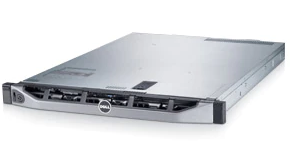
\includegraphics{imatges/serverR320.png}
\end{enumerate}

Especificacions

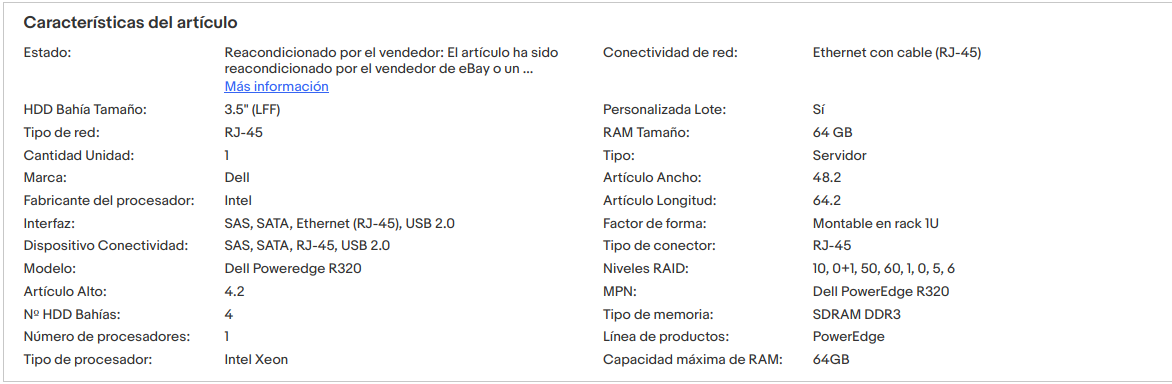
\includegraphics{imatges/server_hp.png} \href{https://i.dell.com/sites/csdocuments/Shared-Content_data-Sheets_Documents/ja/jp/Dell-PowerEdge-R320Technical-Guide.pdf}{Documentació del model}, si va avant, mirar posar un ssd, no està clar. No veig comp amb \href{https://ubuntu.com/certified?category=Server\&vendor=Dell+EMC\&offset=20}{ubuntu}, igual mirar altre server.

Nota: Si és compatible.

\emph{Dimensions servidor} 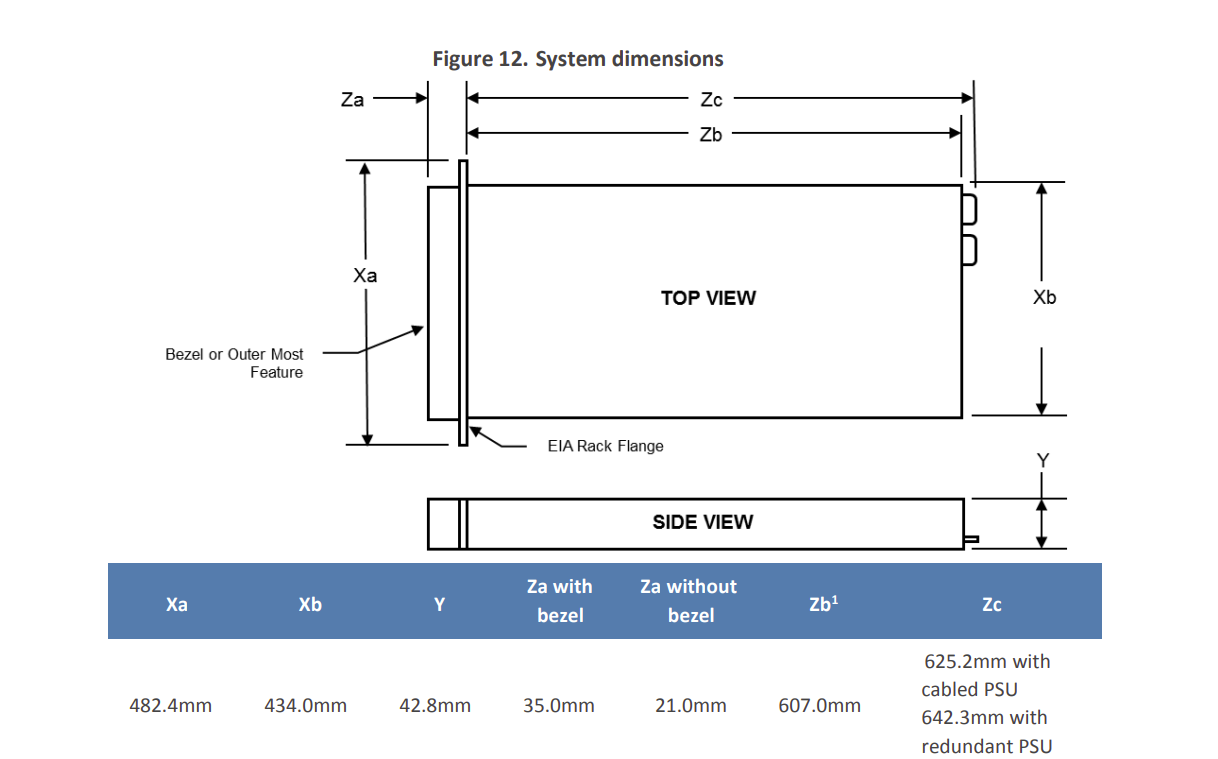
\includegraphics{imatges/dimserver.png}

Cal buscar un rack que done les dimensions.

\href{https://www.dell.com/support/contents/es-es/videos/videoPlayer/os-deployment-installing-microsoft-windows-2012-r2-operating-system-by-using-lifecycle-controller/6079802988001}{video de instal-lació}

\begin{enumerate}
\def\labelenumi{\arabic{enumi}.}
\setcounter{enumi}{1}
\item
  Discs durs, admet segons documentació 4 SATA de 4Gb. Recomane \href{https://www.pcbox.com/st4000dm004-seagate-barracuda--st4000dm004-4000gb-3-5--serial-ata-iii/p}{SEAGATE Barracuda ST4000DM004 4000GB 3.5 Serial ATA III} \href{https://www.amazon.es/Seagate-Barracuda-Disco-Interno-cach\%C3\%A9/dp/B0713R3Y6F/ref=sr_1_5?__mk_es_ES=\%C3\%85M\%C3\%85\%C5\%BD\%C3\%95\%C3\%91\&crid=JR7AGWGKGDES\&keywords=hd\%2Bsata\%2B4tb\&qid=1651315567\&sprefix=hd\%2Bsata\%2B4tb\%2Caps\%2C93\&sr=8-5\&th=1}{amazon} \href{https://www.amazon.com/Seagate-BarraCuda-Internal-Drive-3-5-Inch/dp/B07D9C7SQH/ref=sr_1_1_sspa?keywords=4tb\%2Bsata\%2Bhard\%2Bdrive\&qid=1651315472\&sr=8-1-spons\&spLa=ZW5jcnlwdGVkUXVhbGlmaWVyPUExSldCREdJVFMzRUtNJmVuY3J5cHRlZElkPUEwNTc5NTIwMlRYQzQ0OTA0QVNDOCZlbmNyeXB0ZWRBZElkPUEwNjQxNjk2MjU1VkFSWjM1NVA4MiZ3aWRnZXROYW1lPXNwX2F0ZiZhY3Rpb249Y2xpY2tSZWRpcmVjdCZkb05vdExvZ0NsaWNrPXRydWU\&th=1}{amazon usa} Farien falta 3 per a fer el Raid, estaria bé tindre un de reserva per si falla, un disc, i regenerar el raid. Si s'adquiriren 4, es pot fer un Raid 6 que té dos de paritat. Ell soles es regenera.

  Tindríem dos discs de 4\,TB, que serien 8Gb d'espai efectiu i un de paritat.
\item
  Preguntar a Toni el Hypervisor més adequat.
\item
  Un Sai, mirar potencia, quan es decideixen el server. Es pot posar també una segona font al servidor. Buscar preus.
\item
  Un armari \href{https://www.pccomponentes.com/microconnect-armario-rack-19-6u-600x600mm-negro}{Rack} per al servidor i el switch.
\item
  Switch, preguntar a Toni sobre els cisco, reciclats.
\item
  \href{https://www.pccomponentes.com/buscar/?query=patch\%20panel\&or-relevance}{Patch panel}, cables, connectors rj45 \ldots{}
\end{enumerate}

\hypertarget{avantatges}{%
\section{Avantatges}\label{avantatges}}

La idea és muntar un servidor de Nextcloud, per l'emmagatzematge dels fitxers de la sala. Aprofitar aquest entorn per a posar també, treball en grup de documents amb \href{https://www.collaboraoffice.com/}{Collabora}, o si els agrada més el plug de MS office en línia. Encara que hi ha altres solucions dins el mateix Nextcloud per a fer treball en grup. Provar d'integrar \href{https://etherpad.org/}{Etherpad} en Nextcoud, en un Docker i afegir-lo al menu.

Crear grups de treball on es puga compartir fitxers, com per exemple, un de redactors de la revista, on puguen discutir sobre els articles a publicar. Un altre per als treballadors, per a l'administració, inclús es pot fer grups per a les companyies convidades per fer els seus espectacles.

Es pot aprofitar el sistema de Talk que té, per poder fer comunicacions entre els membres de l'empresa, entre el comandament de llums i el vestuari dels actors, entre redactors i director de la revista per discutir els articles\ldots{} Amb el seu servei de comunicacions privat.

\hypertarget{pfsense-1}{%
\subsection{Pfsense}\label{pfsense-1}}

Primer que res, hem de posar un sistema de seguretat o \href{https://en.wikipedia.org/wiki/DMZ_\%28computing\%29}{DZM}, o farem amb \href{https://www.pfsense.org/}{Pfsense}, mitjançant una VM en el servidor.

\begin{rmdtip}{Tip}

A l'hora de configurar el pfsese tenim dues opcions.

\begin{itemize}
\tightlist
\item
  Fer una VPN
\item
  Exposar els ports que volem, el 443
\end{itemize}

\end{rmdtip}

El millor seria fer una VPN, pero per l'administració de després pot ser un poc complicat per a l'empresa, si no tenen un administrador.

Ens decantarem per exposar el port 443.

La configuració la posaré en un apartat posterior. Configurarem el DHCP, les vpn, el DDNS i el DNS en aquesta màquina virtual, que sera el cor de la xarxa.

\hypertarget{ddns}{%
\subsection{DDNS}\label{ddns}}

Traure conter en un DNS dinàmic. En fer la instal.lació de Nexctcloud VM pels scripts de guithub, ja en s crea un en dedyn.io, mirar altres opcions. A més ens crea un certificat d'aquest domini en Lets encrypt. Mirar la possibilitat de la creació d'un subdomini en el domini de l'empresa, preguntar el dns suporta subdominis, i qui dona el servei.

\hypertarget{nextcloud-1}{%
\subsection{Nextcloud}\label{nextcloud-1}}

Fem servir els \href{https://github.com/nextcloud/vm.git}{scripts} de instal.lacio, que afegeixen millores de seguretat i rendiment.

\begin{rmdtip}{Tip}
Fer un lvm en el RAID 5 del servidor i donar format ZFS, la VM de Nextcloud en el ssd si el podem posar o en el disc de les VM

\end{rmdtip}

\hypertarget{accuxe9s-point-del-wifi}{%
\section{Accés point del wifi}\label{accuxe9s-point-del-wifi}}

En una altra VM posar el software que controla les antenes del wifi

\hypertarget{servidor-de-disc-per-al-video}{%
\section{Servidor de disc per al video}\label{servidor-de-disc-per-al-video}}

Normalment les càmeres ip funcionen en un servidor d'ftp on es guarden les gravacions. En el Raid 5 fem una altra partició lvm d'espai per aquest propòsit, i posem un servidor de sftp en una altra VM on també tindrem el servidor web. Aquesta partició de dades la podem compartir per xarxa amb la VM de Nextcloud on podem muntar medis externs i compartir en els usuaris que volem, par a què es puga muntar també en ella, perquè els usuaris puguen veure les gravacions, sols dret de lectura.

\hypertarget{pressupost-1}{%
\section{Pressupost}\label{pressupost-1}}

\begin{itemize}
\tightlist
\item
  Servidor 265 + iva = 300 euros
\item
  Hd 90 x 3 =270 euros
\item
  Rack 150 euros
\item
  switch ? al voltant de 300 euros
\item
  Antena wifi 150, per antena, si són dos, el segon pot ser d'uns 100 euros.
\item
  Patch panel 25 euros.
\item
  \href{https://www.pccomponentes.com/bobina-cable-utp-cat6-100-mts-negro}{Cables} cat6 60 euros 100 Mts, \href{https://www.pccomponentes.com/digitus-roseta-empotrable-cat6-2-x-rj45-angulo-hembra}{rosetes} 7 euros, \href{https://www.pccomponentes.com/equip-conector-rj45-cat6-100-unidades}{Rj 45} 20 euros (100 unitats)
\item
  Imprevistos 15\%
\item
  3\%, el 3\% clar.
\end{itemize}

\textbf{Total, crec que al voltant de 1500 euros, està fet.}

Càmeres ip, el que vulgueu gastar, de 2500 una amb cmos sony, o per 450 una \href{https://aidaimaging.com/hd-ndi-200/}{Aida HD-NDI-200}, amb una lent fixa, es posa enfocat a l'infinit, amb una lent lluminosa, en gran profunditat de camp, i arreglat. \href{https://www.youtube.com/watch?v=khAv4d11J3g}{video} \href{https://www.youtube.com/watch?v=q8G6seZMzqU}{video poca llum}, \href{https://www.youtube.com/watch?v=3zD6n6GNAuA}{atre}, o es pot provar en càmeres ip de cctv, que per 100 euros hi ha que no estan malament, El problema és la poca llum de la sala. I l'aberració esfèrica que es veu en alguns videos de youtube, deu ser cosa de l'ull de peix que posen per ampliar el camp de visió. Convertidor a ndi, es pot posar per convertir el senyal de la camera HDMI a ndi, o es pot fer en un pc mitjanament potent i el software de DNI. \href{https://support.networkoptix.com/hc/en-us/articles/360010535793-Ubuntu-Linux-OS-Installation-Guide}{Nx Witness VMS} \href{https://www.digitalocean.com/community/tutorials/how-to-set-up-a-video-streaming-server-using-nginx-rtmp-on-ubuntu-20-04}{nginx streamer video} \href{https://shinobi.video/}{Shinobi} El recomanat

\hypertarget{pfsense-2}{%
\chapter{pfSense}\label{pfsense-2}}

\emph{Utilitzem \href{https://docs.netgate.com/pfsense/en/latest}{pfsense} com a cor de la xarxa}

El projecte pfSense® és una distribució personalitzada gratuïta de codi obert de FreeBSD dissenyada per utilitzar-la com a tallafoc i encaminador gestionada completament per una interfície web fàcil d'utilitzar, el programari pfSense inclou una llarga llista de funcions relacionades. El sistema de paquets pfSense permet una major expansió sense afegir vulnerabilitats de seguretat potencials a la distribució base.

\hypertarget{per-a-quuxe8-el-farem-servir}{%
\section{Per a què el farem servir}\label{per-a-quuxe8-el-farem-servir}}

\begin{itemize}
\item
  \emph{Tallafocs perimetrals}, pfSense admet xarxes que requereixen diverses connexions a Internet, diverses xarxes LAN i diverses xarxes DMZ. De moment soles configurarem una WAN, pero estarà preparat pel seu escalat si fera falta en un futur, donar més amplada de banda o redundància de connexió a internet.
\item
  \emph{Encaminador LAN}, per connectar diversos segments de xarxa interna amb VLAN configurades amb troncal 802.1Q.
\item
  \emph{Dispositiu VPN}, com a dispositiu de xarxa privada virtual independent afegeix capacitats VPN sense interrompre la infraestructura del tallafoc existent i inclou diversos protocols VPN.
\item
  \emph{Dispositiu de servidor DHCP}, permet que un dispositiu com el programari pfSense® assigne dinàmicament adreces IP als clients des d'un grup d'adreces predefinits. DHCP també envia informació de configuració als clients, com ara una passarel·la, servidors DNS, nom de domini i altres paràmetres útils.
\item
  \emph{DNS resolver}, el gastarem com a DNS primari.
\item
  Portal captiu, possibilitat de fer un \emph{Hotspot} per a la wifi pública. Obliga els usuaris a autenticar-se abans de concedir accés a Internet. Quan siga possible, el tallafoc presenta automàticament una pàgina web d'inici de sessió en la qual l'usuari ha d'introduir credencials com ara un nom d'usuari/contrasenya, un codi de val o un simple acord de clic.
\item
  \emph{DDNS}, per a configuració del DNS dinàmic i la renovació de credencials.
\end{itemize}

\hypertarget{requeriments}{%
\section{Requeriments}\label{requeriments}}

La distribució de programari pfSense® és compatible amb la majoria de maquinari compatible amb FreeBSD. Les versions actuals del programari pfSense són compatibles amb el maquinari d'arquitectura de 64 bits (amd64, x86-64)

\textbf{Requisits mínims}

\begin{itemize}
\item
  CPU compatible amb amd64 (x86-64) de 64 bits
\item
  1 GB o més de RAM, El propi sistema operatiu, juntament amb altres serveis, requerirà almenys 175-256 MB de RAM addicional i possiblement més segons les funcions utilitzades. Els tallafocs en entorns que requereixen un gran nombre d'estats simultanis han de tenir suficient RAM per a contenir la taula d'estats. Cada estat necessita aproximadament 1 KB de RAM. Cada connexió a través del tallafoc consumeix dos estats: un entrant al tallafoc i un altre que surt del tallafoc.
\item
  Unitat de disc de 8 GB o més (SSD, HDD, etc.)
\item
  Una o més targetes d'interfície de xarxa compatibles, \href{https://www.freebsd.org/cgi/man.cgi?query=bge\&sektion=4\&format=html}{Broadcom 5720}, amb driver bge.
\end{itemize}

\begin{rmdwarn}{Perill}
Problemes específics de la targeta Broadcom bce, fer el que recomana el \href{https://docs.netgate.com/pfsense/en/latest/hardware/tune.html\#broadcom-bge-4-cards}{manual}, La del servidor recomanat és bge, no hauria de tindre problemes.

\end{rmdwarn}

\begin{itemize}
\item
  Opcional, Suport de l'accelerador criptogràfic. el servidor recomanat te \href{https://i.dell.com/sites/csdocuments/Shared-Content_data-Sheets_Documents/ja/jp/Dell-PowerEdge-R320Technical-Guide.pdf}{AES-NI} pag. 17 del manual. Recomanat per a VPN siga més fluid, i no sature la CPU. No cal seleccionar res perquè OpenVPN utilitze AES-NI, natiu.
\item
  Unitat USB d'arrencada o unitat òptica d'alta capacitat (DVD o BD) per a la instal·lació inicial
\end{itemize}

\hypertarget{installaciuxf3}{%
\section{Instal·lació}\label{installaciuxf3}}

Mitjan un dispositiu \href{https://www.netgate.com/pfsense-plus-software/how-to-buy\#appliances}{Netgate} o viralitzant que és el que gastarem. Descarreguem la \href{https://www.pfsense.org/download/}{imatge} AMD64 ISO Estem en fase de proves, farem l'instal.lació en Virtual Box.

Configuració de prova VBox

\begin{figure}
\centering
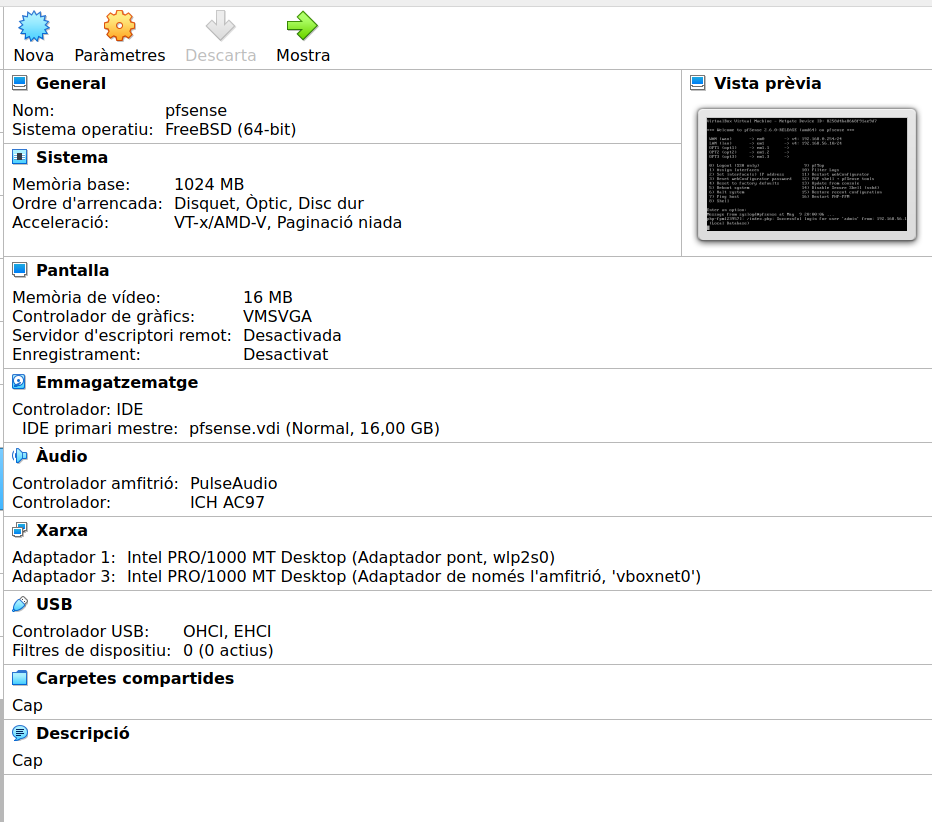
\includegraphics{imatges/pfSense_vbox.png}
\caption{pfSense VBox}
\end{figure}

\begin{rmdnote}{Nota}
Recomanem utilitzar hipervisors de tipus 1 per a ús de producció. Els hipervisors de tipus 2 com ara VirtualBox o VMware Workstation funcionen bé per a les proves, però eviteu utilitzar-los per a funcions de producció sempre que sigui possible.

\end{rmdnote}

La forma d'instal.lació és com qualsevol VM, hem baixat la versió 2.6

\begin{rmdnote}{Nota}
En l'opció 2 definim les ip de les targetes, pfSense les detecta automàticament, pero les he canviat per les proves. En el meu cas de moment és 192.168.0.254 per a la WAN, la que comunica en internet, i la interna LAN 192.168.56.10 per comunicar en vboxnet amb l'amfitrió, no són definitives, la LAN es recomana ser una 172 si es vol fer VPN.

\end{rmdnote}

mirar lo de la ip de la WAN, ara es DHCP, canviar la nota

El que tenim en consola

\begin{Shaded}
\begin{Highlighting}[]
\ExtensionTok{VirtualBox}\NormalTok{ Virtual Machine }\AttributeTok{{-}}\NormalTok{ Netgate Device ID: 8258d4ba8668f91ae9d7}

\ExtensionTok{***}\NormalTok{ Welcome to pfSense 2.6.0{-}RELEASE }\ErrorTok{(}\ExtensionTok{amd64}\KeywordTok{)} \ExtensionTok{on}\NormalTok{ pfsense }\PreprocessorTok{***}

 \ExtensionTok{WAN} \ErrorTok{(}\ExtensionTok{wan}\KeywordTok{)}       \ExtensionTok{{-}}\OperatorTok{\textgreater{}}\NormalTok{ em0        }\AttributeTok{{-}}\OperatorTok{\textgreater{}}\NormalTok{ v4: 192.168.0.254/24}
 \ExtensionTok{LAN} \ErrorTok{(}\ExtensionTok{lan}\KeywordTok{)}       \ExtensionTok{{-}}\OperatorTok{\textgreater{}}\NormalTok{ em1        }\AttributeTok{{-}}\OperatorTok{\textgreater{}}\NormalTok{ v4: 192.168.56.10/24}

 \ExtensionTok{0}\ErrorTok{)} \ExtensionTok{Logout} \ErrorTok{(}\ExtensionTok{SSH}\NormalTok{ only}\KeywordTok{)}                  \ExtensionTok{9}\ErrorTok{)} \ExtensionTok{pfTop}
 \ExtensionTok{1}\ErrorTok{)} \ExtensionTok{Assign}\NormalTok{ Interfaces                 10}\ErrorTok{)} \ExtensionTok{Filter}\NormalTok{ Logs}
 \ExtensionTok{2}\ErrorTok{)} \ExtensionTok{Set}\NormalTok{ interface}\ErrorTok{(}\ExtensionTok{s}\KeywordTok{)} \ExtensionTok{IP}\NormalTok{ address       11}\ErrorTok{)} \ExtensionTok{Restart}\NormalTok{ webConfigurator}
 \ExtensionTok{3}\ErrorTok{)} \ExtensionTok{Reset}\NormalTok{ webConfigurator password    12}\ErrorTok{)} \ExtensionTok{PHP}\NormalTok{ shell + pfSense tools}
 \ExtensionTok{4}\ErrorTok{)} \ExtensionTok{Reset}\NormalTok{ to factory defaults         13}\ErrorTok{)} \ExtensionTok{Update}\NormalTok{ from console}
 \ExtensionTok{5}\ErrorTok{)} \ExtensionTok{Reboot}\NormalTok{ system                     14}\ErrorTok{)} \ExtensionTok{Disable}\NormalTok{ Secure Shell }\ErrorTok{(}\ExtensionTok{sshd}\KeywordTok{)}
 \ExtensionTok{6}\ErrorTok{)} \ExtensionTok{Halt}\NormalTok{ system                       15}\ErrorTok{)} \ExtensionTok{Restore}\NormalTok{ recent configuration}
 \ExtensionTok{7}\ErrorTok{)} \ExtensionTok{Ping}\NormalTok{ host                         16}\ErrorTok{)} \ExtensionTok{Restart}\NormalTok{ PHP{-}FPM}
 \ExtensionTok{8}\ErrorTok{)} \ExtensionTok{Shell}

\ExtensionTok{Enter}\NormalTok{ an option: }
\end{Highlighting}
\end{Shaded}

Connectant via web i tenim: hem d'accedir des de la xarxa LAN, per defecte el tallafoc bloca la GUI des de la WAN.

\begin{figure}
\centering
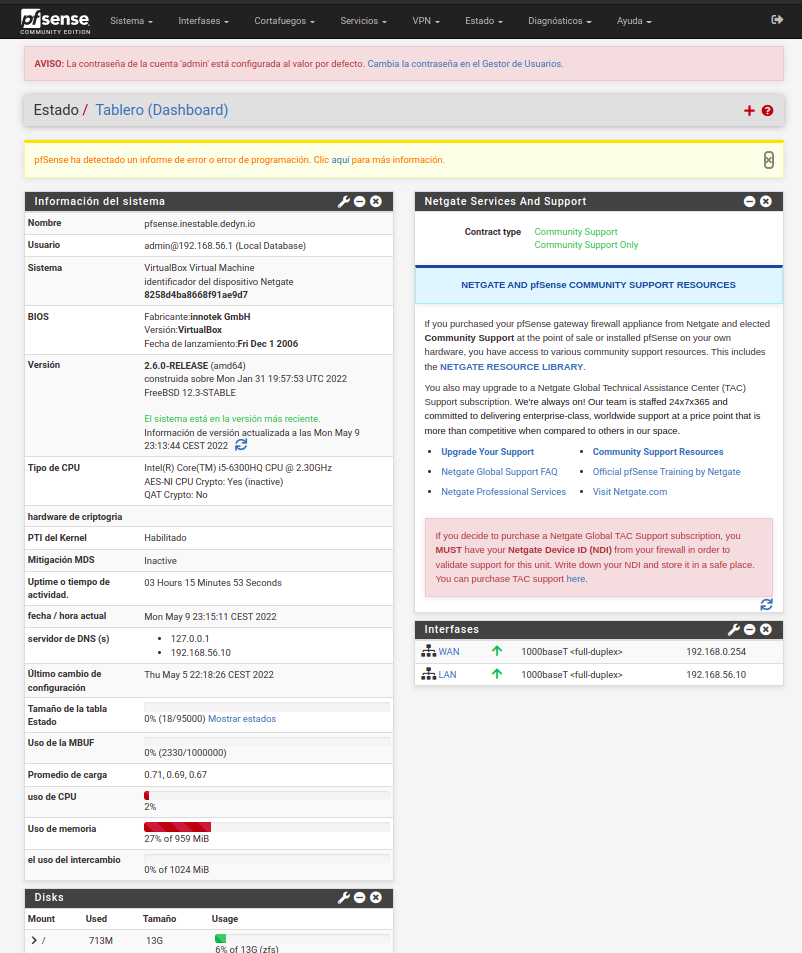
\includegraphics{imatges/pfSense_gui1.png}
\caption{pfsense gui}
\end{figure}

La resta de configuracions es pot fer mitjançant aquesta GUI.

\hypertarget{configuraciuxf3}{%
\section{Configuració}\label{configuraciuxf3}}

Comencem la configuració del pfSense, es pot fer pel wizard o manualment, descriurem breument la manual.

\hypertarget{informaciuxf3-general}{%
\subsection{Informació general}\label{informaciuxf3-general}}

En sistema -\textgreater{} configuració general, donarem nom al host i el domini, així com l'idioma de la GUI, NTP, DNS primari.

El nom del host sera pfsense, i el domini inestable.dedyn.io, ja que em tret un conter en el DDNS de \href{https://desec.io/}{deSEC} amb aquest nom.

\begin{figure}
\centering
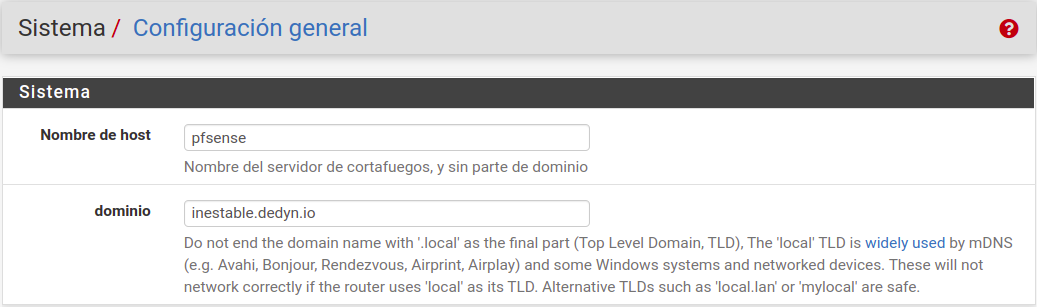
\includegraphics{imatges/pfsense_conf1.png}
\caption{pfsense\_conf1}
\end{figure}

\begin{rmdinfo}{Nota}
El servidor DNS es poden deixar en blanc si el DNS Resolver està actiu mitjançant la configuració predeterminada. La configuració predeterminada té el DNS Resolver actiu en mode de resolució (no en mode de reenviament), quan s'estableix d'aquesta manera, el DNS Resolver no necessita reenviar servidors DNS, ja que es comunicarà directament amb els servidors DNS arrel i altres servidors DNS autoritzats. Per forçar el tallafoc a utilitzar aquests servidors DNS configurats, activeu el mode de reenviament al DNS Resolver. Mes tard podem fer un ns2 replica i configurar aquesta opció dels dos servidors.

\end{rmdinfo}

\hypertarget{configuraciuxf3-wan}{%
\subsection{Configuració WAN}\label{configuraciuxf3-wan}}

Aquesta és la xarxa externa que s'enfronta a l'ISP o a l'encaminador amunt, de manera que l'assistent ofereix opcions de configuració per admetre diversos tipus de connexió d'ISP comuns.

\begin{itemize}
\tightlist
\item
  Tipus WAN, El tipus seleccionat ha de coincidir amb el tipus de WAN requerit per l'ISP, l'opció predeterminada és DHCP a causa del fet que és el més comú, aquesta configuració permet que un tallafoc ``Just Work'' sense configuració addicional.
\end{itemize}

\begin{figure}
\centering
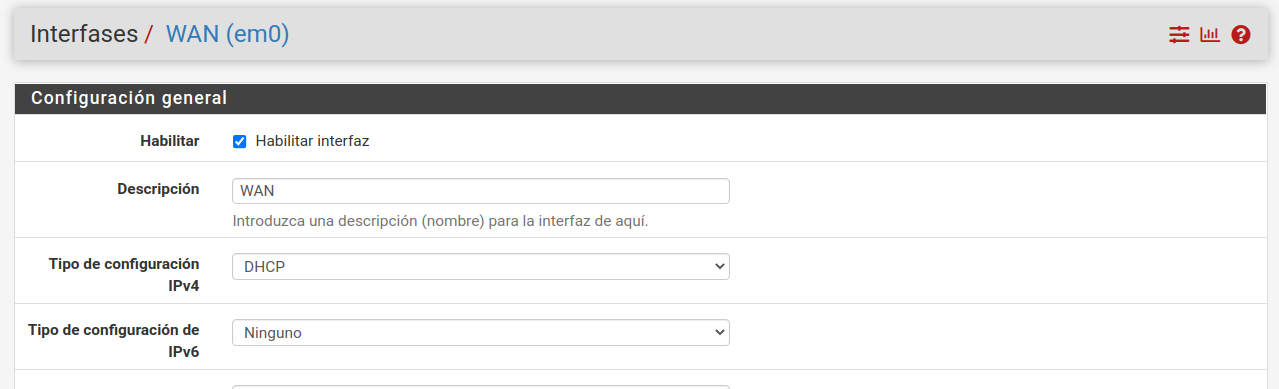
\includegraphics{imatges/pfsense_WAN.png}
\caption{Configuracio WAN}
\end{figure}

\begin{rmdtip}{Nota}
Seleccionem en el tipus DHCP i ques proporcione una ip l'encaminador, la podríem posar en estàtica i ens apareix un nou menu on li donaríem una ip en la mateixa xarxa que l'encaminador, una màscara i la direcció del gateway, l'encaminador.

\end{rmdtip}

\hypertarget{bloqueja-les-xarxes}{%
\subsubsection{Bloqueja les xarxes}\label{bloqueja-les-xarxes}}

\begin{itemize}
\tightlist
\item
  privades RFC 1918, Bloqueja les connexions procedents de xarxes privades registrades d'entrar a la interfície WAN.
\item
  Bogon, el tallafoc bloqueja l'entrada de trànsit si prové d'espai IP reservat o no assignat que no s'hauria d'utilitzar. La llista de xarxes bogon s'actualitza periòdicament en segon pla i no requereix cap manteniment manual.
\end{itemize}

Seleccionem els dos bloquejos.

\begin{figure}
\centering
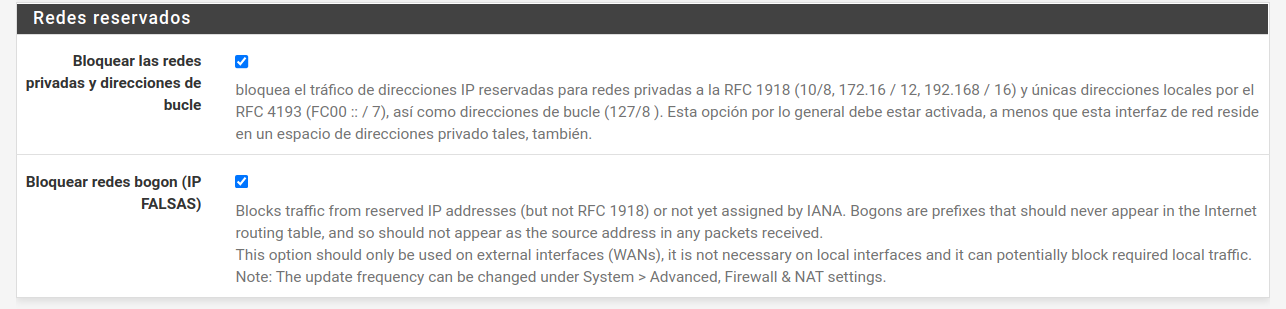
\includegraphics{imatges/pfsense_reservado.png}
\caption{Bloqueja les xarxes}
\end{figure}

\hypertarget{configuraciuxf3-lan}{%
\subsection{Configuració LAN}\label{configuraciuxf3-lan}}

Tenim dues opcions

\begin{itemize}
\tightlist
\item
  Si aquest tallafoc no es connecta a cap altra xarxa mitjançant VPN, és possible que la 192.168.1.0/24 xarxa predeterminada siga acceptable.
\item
  Si aquesta xarxa s'ha de connectar a una altra xarxa, mitjançant VPN des d'ubicacions remotes, triarem un rang d'adreces IP privades molt més fosc que el predeterminat comú de 192.168.1.0/24. L'espai IP dins del 172.16.0.0/12 bloc d'adreces privades RFC 1918 és generalment el que s'utilitza amb menys freqüència, així que trieu alguna cosa 172.16.x.x per 172.31.x.x evitar les dificultats de connectivitat VPN.
\end{itemize}

\begin{rmdwarn}{Nota}
Si un client remot es troba en un punt d'accés sense fil utilitzant 192.168.1.x (molt comú), el client no es podrà comunicar a través de la VPN. En aquest cas, 192.168.1.x és la xarxa local del client al punt d'accés, no la xarxa remota a través de la VPN.

\end{rmdwarn}

\begin{figure}
\centering
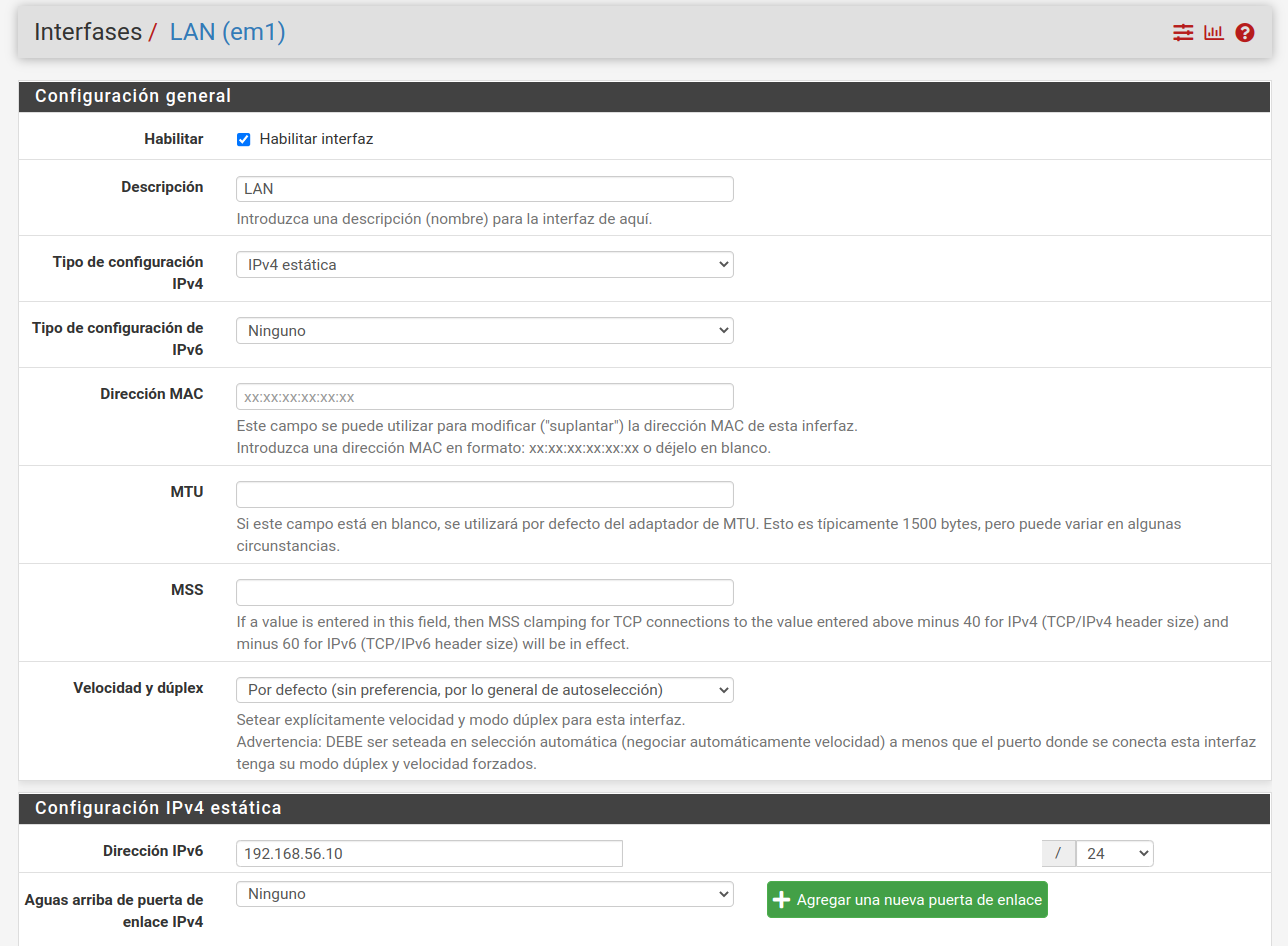
\includegraphics{imatges/pfsense_LAN.png}
\caption{Configuració LAN}
\end{figure}

\begin{rmdnote}{Nota}
De moment ho deixarem en la 192.168.56.x per acabar la integració de tots els serveis, i ho modificarem en implementar la VPN.

\end{rmdnote}

\hypertarget{configuraciuxf3-de-interfaces}{%
\subsection{Configuració de interfaces}\label{configuraciuxf3-de-interfaces}}

\hypertarget{vpn}{%
\section{vpn}\label{vpn}}

Les VPN d'accés remot permeten als usuaris connectar-se de manera segura a una xarxa des de qualsevol lloc on hi haja una connexió a Internet disponible. Per oferir als empleats la possibilitat de treballar des de casa. També pot permetre als contractistes o venedors l'accés temporal a una xarxa. Amb la proliferació de telèfons intel·ligents, els usuaris tenen la necessitat d'accedir de manera segura als serveis interns des dels seus telèfons mitjançant una VPN d'accés remot.

Les VPN d'accés remot es poden configurar de manera que passe tot el trànsit del sistema client a través de la VPN, té un impacte en el rendiment, LA farem soles per accedir als serveis de l'empresa.

\hypertarget{autenticaciuxf3}{%
\subsection{Autenticació}\label{autenticaciuxf3}}

Possibilitats

\begin{itemize}
\tightlist
\item
  IPsec
\item
  OpenVPN
\item
  WireGuard (No recomanable)
\end{itemize}

L'ús d'OpenVPN amb certificats, autenticació TLS i autenticació d'usuari és el mètode més segur i més senzill d'implementar. El xifratge es veu compromès si es comprometen les claus privades de l'estructura PKI, tot i que l'ús de múltiples factors com l'autenticació TLS a la part superior de la PKI pot mitigar part del perill.

OpenVPN requereix l'ús de certificats per a l'accés remot a la majoria d'entorns, que inclou la seua pròpia corba d'aprenentatge i pot ser una mica difícil de gestionar. Hi ha un assistent per gestionar les configuracions d'accés remot d'OpenVPN més habituals i els paquets d'exportació de clients d'OpenVPN faciliten el procés de posar en funcionament els clients.

OpenVPN té \href{https://openvpn.net/vpn-client/}{clients} disponibles per a Windows, Mac OS X, tots els BSD, Linux, Solaris i Windows Mobile, \href{https://play.google.com/store/apps/details?id=de.blinkt.openvpn}{Android}, \href{https://apps.apple.com/us/app/openvpn-connect/id590379981}{iOS}, però el client no ve preinstal·lat en cap d'aquests sistemes operatius. En funció del desplegament, els clients mòbils (Accés remot) poden rebre una configuració automàtica en determinats casos, poden rebre automàticament una adreça IP (recomanat 172\ldots) assignada des d'un grup, i es poden enviar nombroses opcions addicionals als clients per controlar el seu comportament des del costat del servidor (encaminament, DNS i molts altres).

\hypertarget{firewall}{%
\subsection{Firewall}\label{firewall}}

OpenVPN és molt compatible amb el tallafoc. Com que utilitza un únic port UDP o TCP i no es veu afectat per les funcions NAT habituals. OpenVPN admet NAT entrant (per exemple, reenviaments de ports) i sortint mitjançant la pestanya OpenVPN del grup i també a les interfícies assignades. L'única dificultat possible és si el protocol i el port en ús estan bloquejats. Quan s'assignen com a interfície, les instàncies d'OpenVPN admeten completament les regles per túnel.

\hypertarget{regles}{%
\subsubsection{Regles}\label{regles}}

L'assistent VPN d'accés remot d'OpenVPN ofereix, crear regles per passar el trànsit i el trànsit WAN a la interfície d'OpenVPN. El trànsit encapsulat dins d'una connexió OpenVPN activa es controla mitjançant regles definides per l'usuari a la pestanya OpenVPN a Firewall \textgreater{} Regles.

Mirar si fem un LDAP

\hypertarget{configuraciuxf3-uxf2ptima-de-xifratge}{%
\subsection{Configuració òptima de xifratge}\label{configuraciuxf3-uxf2ptima-de-xifratge}}

\begin{itemize}
\tightlist
\item
  Utilitzeu maquinari compatible amb AES-NI.
\item
  A la configuració de la Fase 1 (IKE), utilitzeu:

  \begin{itemize}
  \tightlist
  \item
    AES128-GCM amb longitud de clau de 128 bits per a l'algorisme
  \item
    AES-XCBC per al hash, que en aquest cas és efectivament una funció pseudoaleatòria (PRF). Això donarà el màxim rendiment en combinació amb AES128-GCM en maquinari que pot accelerar tots dos (per exemple, AES-NI)
  \end{itemize}
\item
  A la configuració de la Fase 2 (SA infantil), utilitzeu:

  \begin{itemize}
  \tightlist
  \item
    AES128-GCM amb longitud de clau de 128 bits per a l'algorisme
  \item
    No seleccioneu cap algoritme hash. Un algorisme hash no és necessari per a AES-GCM, ja que ja inclou l'autenticació.
  \end{itemize}
\end{itemize}

\hypertarget{udp}{%
\subsection{UDP}\label{udp}}

UDP té menys despeses generals per a les dades tunelades i, si un client ha de retransmetre, no augmentarà el problema retransmetent tant dins com fora del túnel.

\hypertarget{utilitzeu-tls-nomuxe9s-per-a-lautenticaciuxf3}{%
\subsection{Utilitzeu TLS només per a l'autenticació}\label{utilitzeu-tls-nomuxe9s-per-a-lautenticaciuxf3}}

OpenVPN pot utilitzar TLS tant per a l'autenticació com per al xifratge del canal de control. Realitzar el xifratge del canal de control afegeix més sobrecàrrega, que pot augmentar amb molts clients. Si no cal el xifratge del canal de control, considereu utilitzar TLS només per a l'autenticació. Independentment de quina opció escolliu, el trànsit transportat per OpenVPN està xifrat.

\hypertarget{utilitzeu-la-negociaciuxf3-de-xifrat-de-dades}{%
\subsection{Utilitzeu la negociació de xifrat de dades}\label{utilitzeu-la-negociaciuxf3-de-xifrat-de-dades}}

La negociació de xifratge de dades es pot utilitzar per establir preferències de manera que els clients puguen preferir xifrats més eficients quan siga possible, però es poden utilitzar altres quan siga necessari. Estableix primer seleccions d'alta prioritat com ara AES-128-GCM, seguides d'altres com AES-128-CBC.

\hypertarget{tuxfanels-dividits}{%
\subsection{Túnels dividits}\label{tuxfanels-dividits}}

El túnel dividit només envia trànsit per a subxarxes específiques a través de la VPN en lloc d'enviar tot el trànsit. Amb OpenVPN, això es pot fer desmarcant les opcions de redirecció de la passarel·la IPv4/IPv6 i configurant les entrades de xarxes locals IPv4/IPv6. Tanmateix, els clients encara poden anul·lar aquest comportament de forma remota, així que comproveu també les configuracions del client.

\hypertarget{desactiva-la-compressiuxf3}{%
\subsection{Desactiva la compressió}\label{desactiva-la-compressiuxf3}}

La majoria de les dades enviades a través de VPN en entorns moderns ja estan xifrades o no es poden comprimir, cosa que malgasta la CPU quan s'intenta comprimir. A més, vulnerabilitats com VORACLE poden permetre als atacants obtenir informació sobre dades xifrades quan s'han comprimit.

\hypertarget{connexions-duplicades}{%
\subsection{Connexions duplicades}\label{connexions-duplicades}}

Normalment, si un client OpenVPN es connecta utilitzant el mateix nom d'usuari o certificat CN, la connexió anterior es trenca a favor de la nova connexió. Això és més segur, però no permet que cap usuari es connecte diverses vegades. És el cas que tenim, pot estar connectat via web i via app movil.

\hypertarget{utilitzeu-udp-fast-io}{%
\subsection{Utilitzeu UDP Fast I/O}\label{utilitzeu-udp-fast-io}}

Aquesta opció és experimental, però per a aquells que l'han utilitzat, pot resultar en un rendiment molt més elevat.

\hypertarget{augmenta-la-memuxf2ria-intermuxe8dia-denviamentrecepciuxf3}{%
\subsection{Augmenta la memòria intermèdia d'enviament/recepció}\label{augmenta-la-memuxf2ria-intermuxe8dia-denviamentrecepciuxf3}}

La mida de memòria intermèdia predeterminada és segura, però no òptima. Augmentar la mida de la memòria intermèdia fins a 512 KiB a ambdós costats pot augmentar el rendiment.

\hypertarget{openvpn-i-certificats}{%
\subsection{OpenVPN i certificats}\label{openvpn-i-certificats}}

La millor pràctica és utilitzar certificats per a l'accés remot i les VPN de lloc a lloc perquè permet revocar l'accés per a clients o llocs individuals. Idealment, els certificats haurien de ser únics per dispositiu o almenys per usuari. Si un client amb un certificat individual està compromès o l'accés s'ha de revocar per qualsevol altre motiu, simplement revoqueu aquest certificat. No hi ha cap altre client afectat.

La GUI del programari pfSense inclou una interfície de gestió de certificats totalment integrada amb OpenVPN. Les autoritats de certificació (CA) i els certificats de servidor es gestionen al Gestor de certificats a la interfície web, que es troba a Sistema \textgreater{} Gestor de certificats. Els certificats d'usuari també es gestionen a la interfície web, com a part del gestor d'usuaris integrat que es troba a Sistema \textgreater{} Gestor d'usuaris. Els certificats es poden generar per a qualsevol compte d'usuari creat localment al tallafoc, excepte el compte d'administrador predeterminat.

\begin{itemize}
\tightlist
\item
  Peer to Peer (SSL/TLS)
\item
  Peer to Peer (clau compartida)
\item
  Accés remot (SSL/TLS)
\item
  Accés remot (autenticació d'usuari)
\item
  Accés remot (SSL/TLS + autenticació d'usuari)
\end{itemize}

Utilitzarem \emph{Accés remot (SSL/TLS + autenticació d'usuari)}

Aquesta és l'opció més segura disponible. No només obté els avantatges d'altres opcions SSL/TLS, sinó que també requereix un nom d'usuari i una contrasenya del client quan es connecta. L'accés del client es pot eliminar no només revocant el certificat, sinó també canviant la contrasenya. A més, si no es descobreix immediatament una clau compromesa, el perill es redueix perquè és poc probable que l'atacant tinga les claus i la contrasenya.

\hypertarget{mode-de-dispositiu}{%
\subsection{Mode de dispositiu}\label{mode-de-dispositiu}}

OpenVPN es pot executar en un dels dos modes de dispositiu:

\begin{itemize}
\item
  tun: Funciona a la capa 3 OSI i realitza l'encaminament en interfícies punt a punt.
\item
  Toc: Pot funcionar a la capa 2 OSI i pot realitzar tant l'encaminament com el pont si és necessari.
\end{itemize}

Els clients com els que es troben a Android i iOS només admeten el mode \emph{tun} a les aplicacions que la majoria de la gent pot utilitzar. Farem servir aquest mode.

\hypertarget{configuraciuxf3-del-punt-final}{%
\section{Configuració del punt final}\label{configuraciuxf3-del-punt-final}}

\hypertarget{infraestructura}{%
\chapter{Infraestructura}\label{infraestructura}}

\hypertarget{xarxa-per-a-la-sala}{%
\section{Xarxa per a la sala}\label{xarxa-per-a-la-sala}}

Es proposa la següent configuració de xarxa per a la sala.

\begin{itemize}
\tightlist
\item
  Xarxa de CCTV per al \emph{registrament / reproducció en línia} de les obres de teatre.
\item
  Xarxa de wifi, pública i una privada.
\item
  Xarxa interna per als treballadors, amb connexió externa per VPN.
\end{itemize}

Pla de la sala

\begin{figure}
\centering
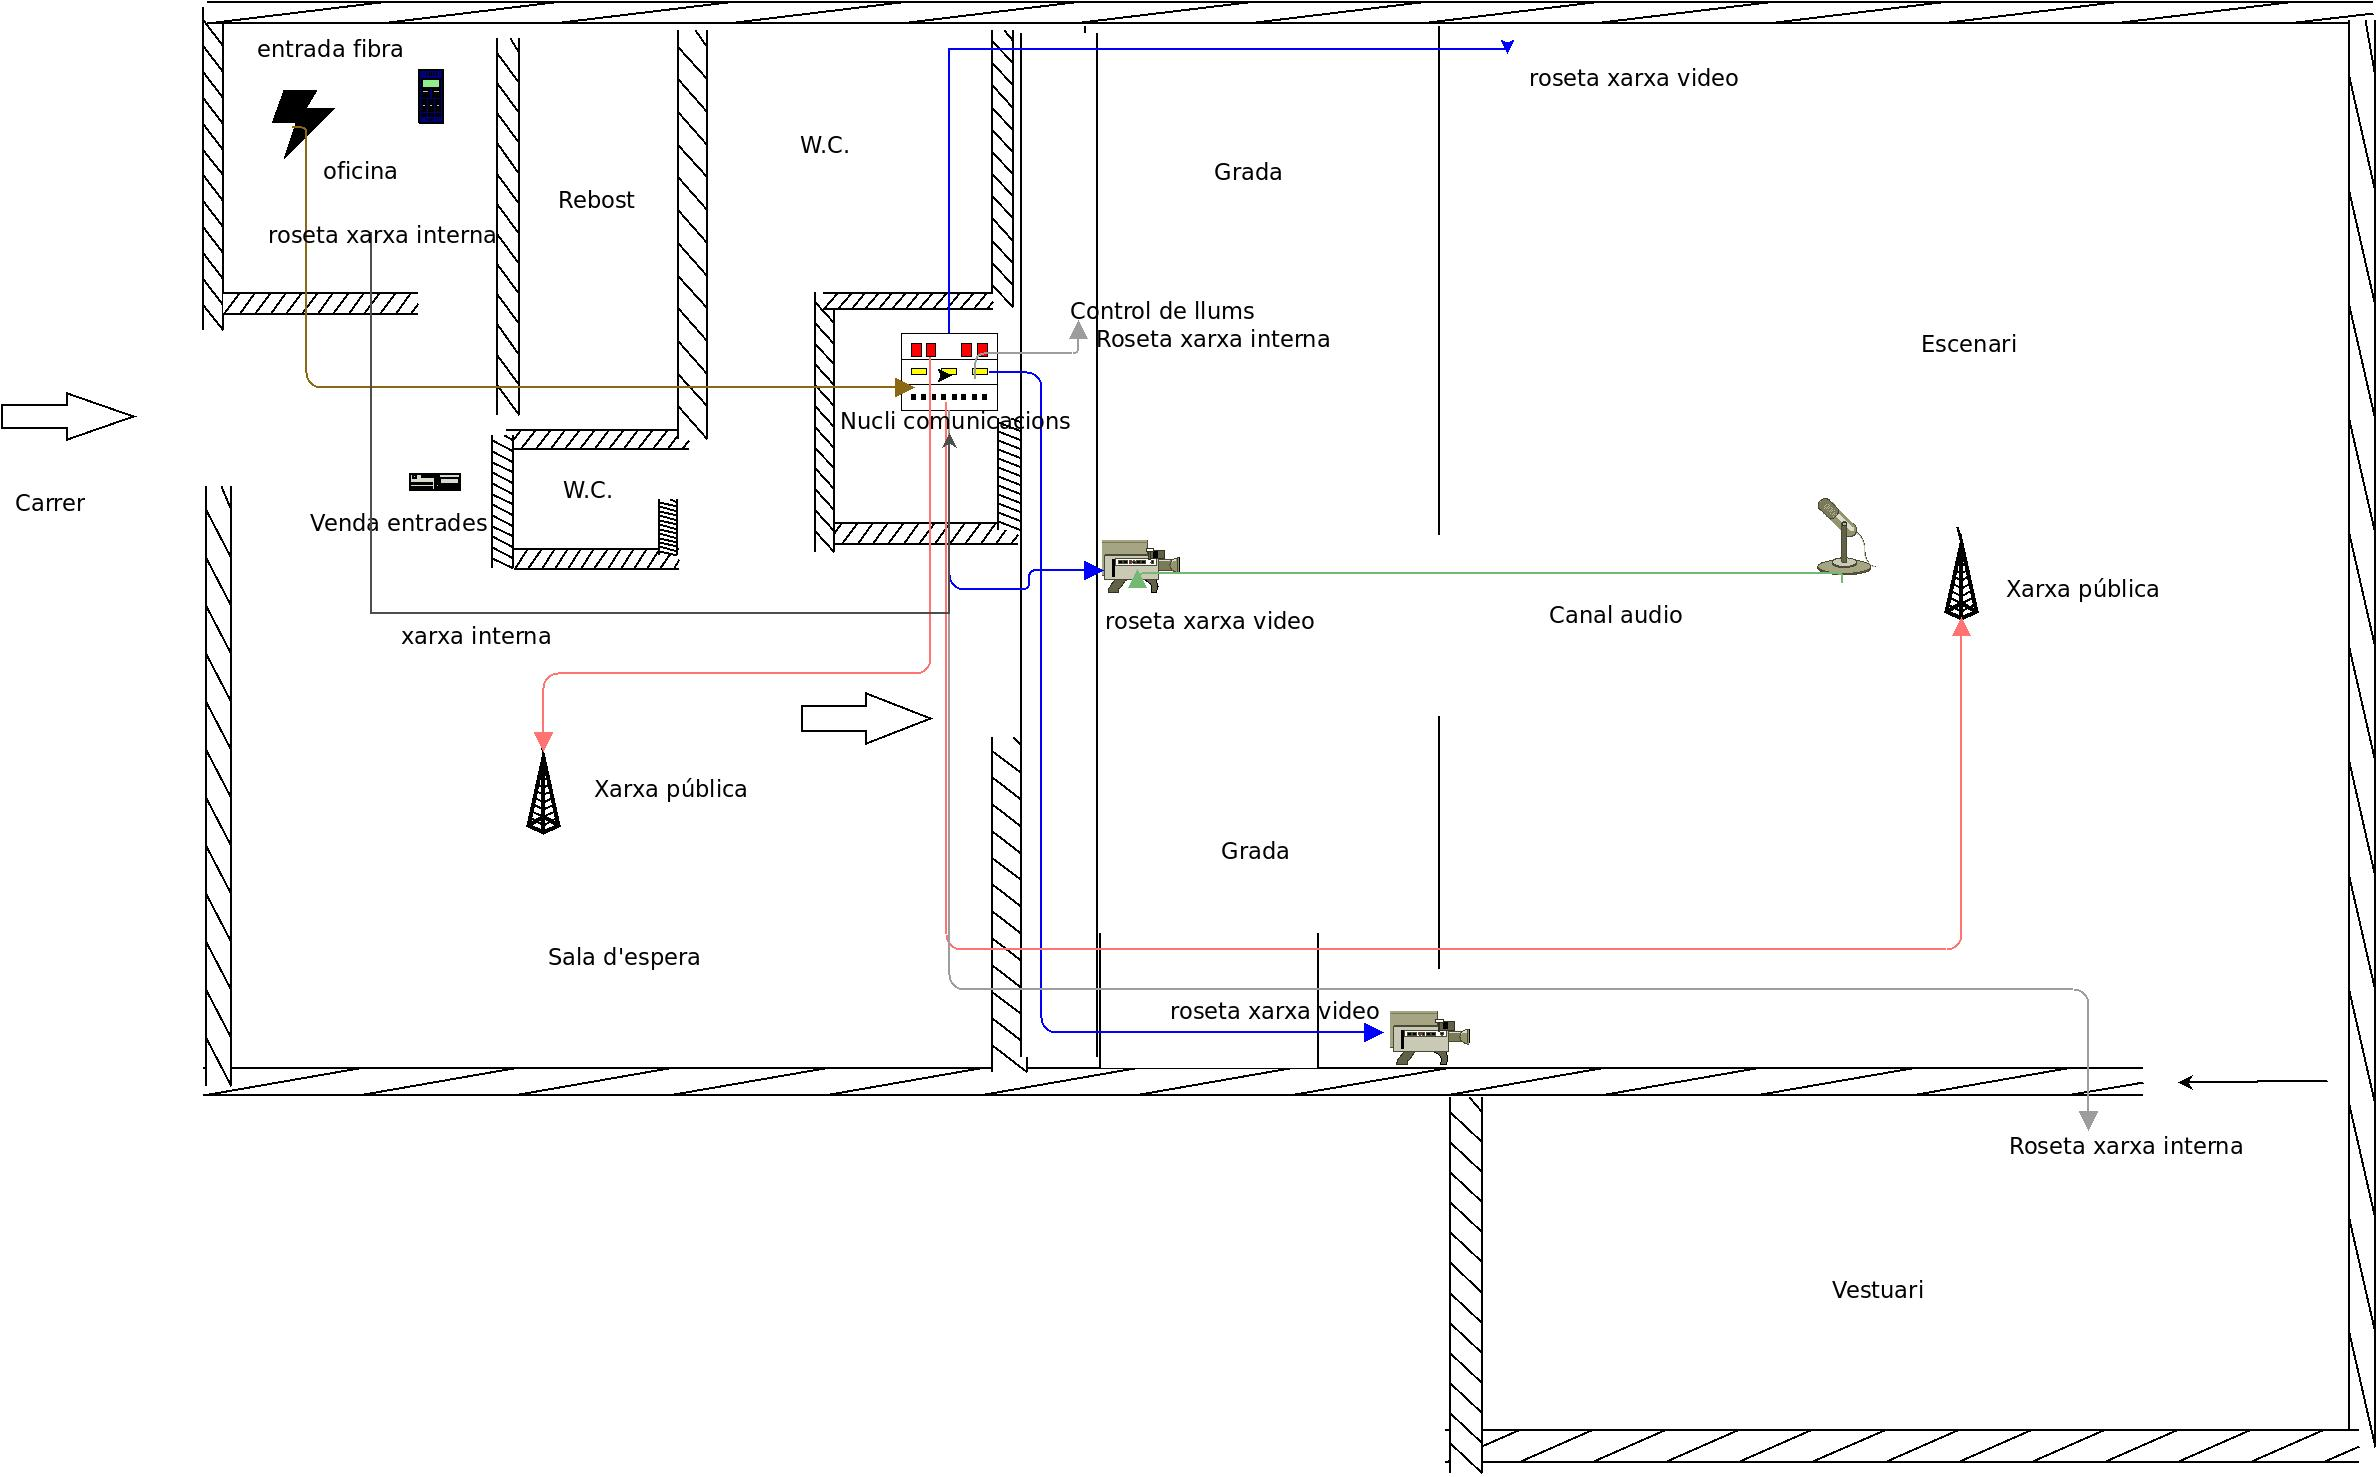
\includegraphics{imatges/teatre.jpeg}
\caption{pla de la sala}
\end{figure}

\hypertarget{descripciuxf3-de-les-instal.lacions}{%
\section{Descripció de les instal.lacions}\label{descripciuxf3-de-les-instal.lacions}}

\hypertarget{oficina}{%
\subsection{Oficina}\label{oficina}}

En l'oficina tenim l'entrada de la connexió de fibra a internet. Des d'aci portem la connexió de xarxa al nucli de comunicacions on tenim la infraestructura de la xarxa, el commutador, el servidor, emmagatzematge de disc. Des del nucli de comunicacions, tornarem una connexió de xarxa cap a l'oficina per donar accés als serveis interns i eixida a internet.

\hypertarget{sala-despera}{%
\subsection{Sala d'espera}\label{sala-despera}}

En aquest espai, tenim l'ordinador de venda d'entrades al que li donarem connexió, siga directa al commutador, per la connexió de l'oficina o el canal wifi privant. En el centre de la sala aniria l'antena wifi PoE connectada al nucli de comunicacions.

\hypertarget{escenari}{%
\subsection{Escenari}\label{escenari}}

\begin{itemize}
\item
  En la sala d'espectacles es traurien 3 connexions de la xarxa video.

  \begin{itemize}
  \tightlist
  \item
    \textbf{Central}, baix de la taula de llums, on es connectara un Camera ip PoE fixa.
  \item
    \textbf{Lateral}, una a cada banda de l'escenari, camera desmuntable que es pot traslladar lateralment segons les necessitats de l'obra representada. Es recomana que aquesta siga del tipus PTZ. Podent ser col.locada a la dreta o l'esquerra de l'escenari.
  \item
    \textbf{Micròfon ambient} que el connectarem a la camera central que es fixa.
  \end{itemize}
\item
  Una connexió per a la xarxa pública, punt per l'antena wifi, al centre del sostre de l'escenari, per donar millor cobertura.
\item
  Un punt de connexió en el vestuari, per comunicació amb la xarxa interna, que pot donar cobertura a l'escenari en cas de conferències, o altres actes que necessiten bona connexió de xarxa.
\end{itemize}

\hypertarget{descripciuxf3-de-les-xarxes}{%
\section{Descripció de les xarxes}\label{descripciuxf3-de-les-xarxes}}

\emph{La configuració de les xarxes, la farem amb 3 VLAN.}

\hypertarget{vlan-video}{%
\subsection{VLAN Video}\label{vlan-video}}

Xarxa interna per la qual anirà el circuit intern de televisió, siga per la reproducció en línia o per fer gravació de les obres en el servidor. Per aquest propòsit, muntarem en el servidor una VM on guardarem les còpies perquè no siga afectat el rendiment per la resta de serveis. Espai que compartirem en la VLAN d'oficina per poder editar el videos posteriorment.

Configurarem accés a aquesta Vlan des del punt wifi de l'escenari, per poder gastar el movil com a camera en les representacions.

\hypertarget{vlan-puxfablica}{%
\subsection{VLAN pública}\label{vlan-puxfablica}}

Xarxa amb connexió a internet per al públic general a través dels punts wifi. La podem configurar amb un portal captiu, amb pfSense, donat d'alta un usuari generic amb permís de connectar a certes hores coincidint en les representacions, canviant el password en cada obra, que oferirem al públic per un codi QR. Es pot aprofitar aquesta connexió per a redirigir als espectadors en un primer moment a un servidor web propi on publicitar properes obres, donar més informació de l'obra que van a veure, o interactuant amb ells via web en el transcurs de la representació.

\hypertarget{vlan-privat}{%
\subsection{VLAN privat}\label{vlan-privat}}

Xarxa amb connexió a internet i als serveis oferits per la sala.

Es donaran els següents accessos.

\begin{enumerate}
\def\labelenumi{\arabic{enumi}.}
\item
  \emph{Taula de llums}, perquè puguen accedir a recursos guardats en el servidor, mantenir comunicació amb el vestuari.
\item
  \emph{Vestuaris}, comunicació o recursos de xarxa a l'escenari.
\item
  \emph{Oficines}, donar accés a recursos del servidor, donar xarxa a telèfon ip instal.lat.
\item
  \emph{Punts wifi}, crearem una segona xarxa amb enquesta Vlan en les antenes wifi de sol accés per als treballadors de la sala.
\end{enumerate}

\hypertarget{servidor-2}{%
\chapter{Servidor}\label{servidor-2}}

Es proposa la compra d'un servidor d'ebay, Per a fer funcionar els serveis que volem oferir.

En el servidor volem implantar els següents serveis:

\begin{itemize}
\item
  Un servidor de disc per a les gravacions de video.
\item
  Servidor de pàgines web, per a le xarxa pública.
\item
  Servidor de Nextcloud.

  \begin{itemize}
  \tightlist
  \item
    Servei d'espai en el núvol.
  \item
    Comunicació entre els membres.
  \item
    Serveis ofimàtics col.laboratius.
  \item
    Agenda, calendari, integrar noves apps generades per a l'empresa.
  \item
    Connectar en enmagtcenament extern per visualitzar o descarregar les gravacions de video.
  \end{itemize}
\item
  Maquina virtual per controlar el wifi de la sala.
\item
  Tallafocs, DNS, DHCP, VPN (pfSense).
\item
  Servidor Ldap per gestionar usuaris Nextcloud i VPN.
\end{itemize}

\hypertarget{hardware}{%
\section{Hardware}\label{hardware}}

\begin{enumerate}
\def\labelenumi{\arabic{enumi}.}
\tightlist
\item
  \href{https://www1.la.dell.com/content/products/productdetails.aspx/poweredge-r320?c=ve\&l=es\&s=corp\&cs=vecorp1}{Servidor}. En \href{https://www.ebay.es/itm/125269454776?hash=item1d2aa42fb8:g:aTIAAOSw3ExiXvm5}{ebai} el podem trobar per uns 250 euros + IVA, amb 64G de ram. 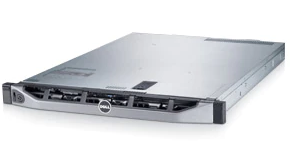
\includegraphics{imatges/serverR320.png}
\end{enumerate}

\textbf{Especificacions}

\begin{figure}
\centering
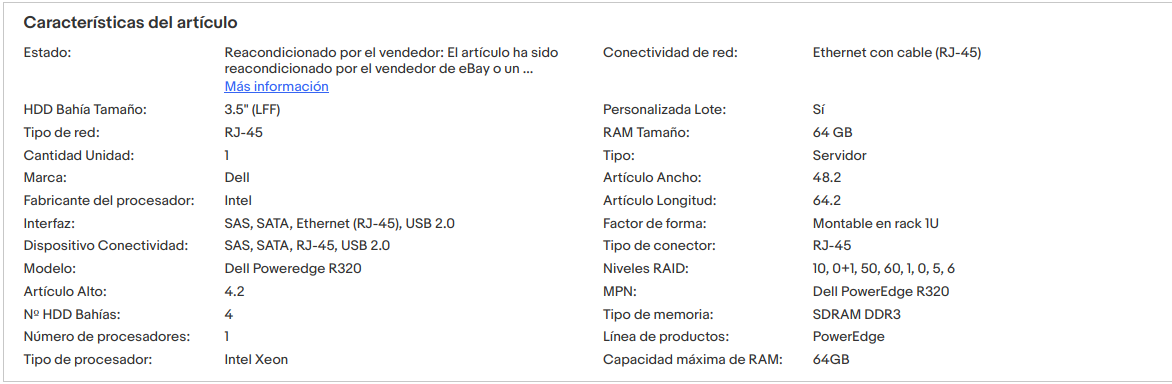
\includegraphics{imatges/server_hp.png}
\caption{server}
\end{figure}

\begin{rmdnote}{}
\href{https://i.dell.com/sites/csdocuments/Shared-Content_data-Sheets_Documents/ja/jp/Dell-PowerEdge-R320Technical-Guide.pdf}{Documentació del model}, i \href{https://www.dell.com/support/home/en-us/product-support/product/poweredge-r320/docs}{manuals}, \href{https://dl.dell.com/topicspdf/poweredge-r320_owners-manual_en-us.pdf}{owner manual} Compatibilitat amb \href{https://ubuntu.com/certified?category=Server\&vendor=Dell+EMC\&offset=20}{ubuntu server}, és compatible amb la versió 14 i posteriors. En la fulla de \href{https://www.dell.com/support/contents/en-us/article/Product-Support/Self-support-Knowledgebase/enterprise-resource-center/server-operating-system-support}{Dell}

\end{rmdnote}

\begin{rmdinfo}{}
És compatible amb la \href{https://linux.dell.com/files/supportmatrix/Ubuntu_Support_Matrix.pdf}{versió 14.04 LTS}, no apareix en la llista, manté la compatibilitat hardware amb les més recents. És un servidor del 2014, pero per als requisits que requerim, pocs usuaris, tràfic limitat, és suficient. A una mala Posem \href{https://www.centos.org/}{CentOS}

\end{rmdinfo}

\emph{Dimensions servidor} 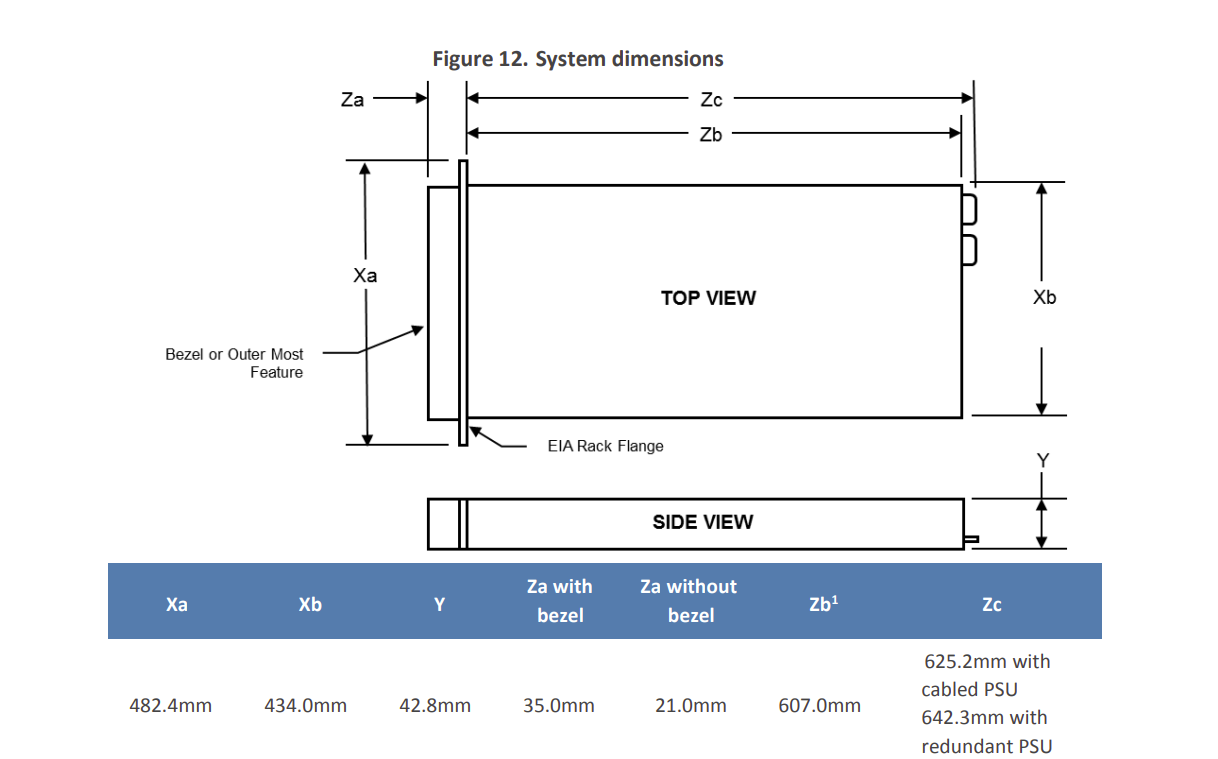
\includegraphics{imatges/dimserver.png}

Cal buscar un rack que done les dimensions.

\href{https://www.dell.com/support/contents/es-es/videos/videoPlayer/os-deployment-installing-microsoft-windows-2012-r2-operating-system-by-using-lifecycle-controller/6079802988001}{video de instal-lació}

\begin{enumerate}
\def\labelenumi{\arabic{enumi}.}
\setcounter{enumi}{1}
\item
  \emph{Discs durs}, admet segons documentació 4 SATA 3.5'\,' o 8 de 2.5'\,' Hot-plug. On fariem RAID per hardware. RAID: Kit RAID H710 Mini 512 MB NV (SAS/ SATA ) - 0/1/5/6/10/50/60 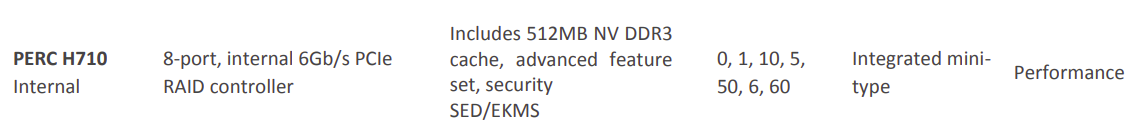
\includegraphics{imatges/ser_h710.png} Caddies: 4 LFF (3.5'') incluidos

  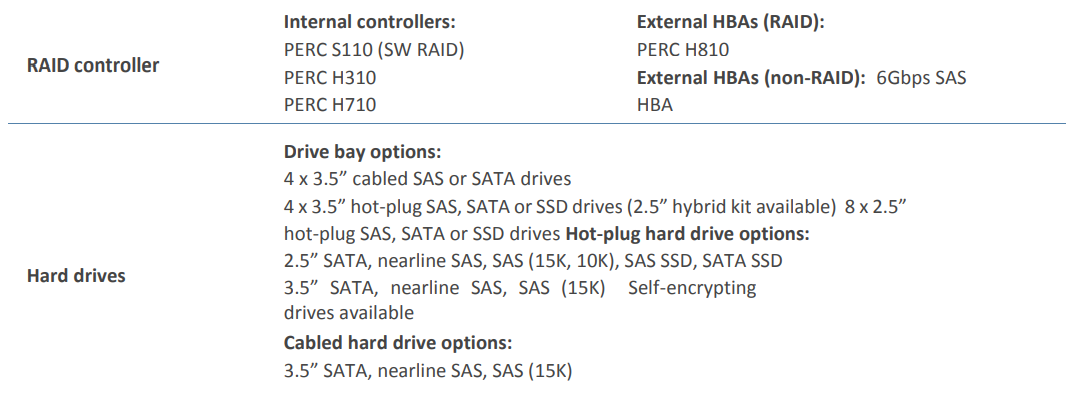
\includegraphics{imatges/ser_hd.png} Recomane \href{https://www.pcbox.com/st4000dm004-seagate-barracuda--st4000dm004-4000gb-3-5--serial-ata-iii/p}{SEAGATE Barracuda ST4000DM004 4000GB 3.5 Serial ATA III} \href{https://www.amazon.es/Seagate-Barracuda-Disco-Interno-cach\%C3\%A9/dp/B0713R3Y6F/ref=sr_1_5?__mk_es_ES=\%C3\%85M\%C3\%85\%C5\%BD\%C3\%95\%C3\%91\&crid=JR7AGWGKGDES\&keywords=hd\%2Bsata\%2B4tb\&qid=1651315567\&sprefix=hd\%2Bsata\%2B4tb\%2Caps\%2C93\&sr=8-5\&th=1}{amazon} \href{https://www.amazon.com/Seagate-BarraCuda-Internal-Drive-3-5-Inch/dp/B07D9C7SQH/ref=sr_1_1_sspa?keywords=4tb\%2Bsata\%2Bhard\%2Bdrive\&qid=1651315472\&sr=8-1-spons\&spLa=ZW5jcnlwdGVkUXVhbGlmaWVyPUExSldCREdJVFMzRUtNJmVuY3J5cHRlZElkPUEwNTc5NTIwMlRYQzQ0OTA0QVNDOCZlbmNyeXB0ZWRBZElkPUEwNjQxNjk2MjU1VkFSWjM1NVA4MiZ3aWRnZXROYW1lPXNwX2F0ZiZhY3Rpb249Y2xpY2tSZWRpcmVjdCZkb05vdExvZ0NsaWNrPXRydWU\&th=1}{amazon usa}

  Farien falta 3 per a fer Raid, estaria bé tindre un de reserva per si falla un disc, i regenerar el Raid. Si en compren 4, es pot fer un Raid 6 que té dos de paritat.

  \texttt{Tindríem\ dos\ discs\ de\ 4\,TB,\ que\ serien\ 8Gb\ d\textquotesingle{}espai\ efectiu\ i\ un\ de\ paritat.}
\item
  RAM: RAM registrada DDR3 de 64 GB. No és la més rapida del mercat, pero suficient per al que necessitem:

  \begin{itemize}
  \tightlist
  \item
    pfSense Min 1GB (imatge oficial), 2GB
  \item
    Servidor HD video 4 GB, si sobra, posar un poc mes, estudiar les demandes de 3 càmeres ip.
  \item
    Nextcloud Min 2GB, recomenat + 8GB
  \item
    Ldap, web server, antenes wifi, Collabora office server, algun altre servei futur, si es vol mail intern \ldots{} (he de pensar si fer una altra VM o repartir en vaires) 4GB.
  \end{itemize}
\item
  UPC: 1x Intel Xeon E5-2440 V2: 8 núcleos, 16 subprocesos, 1,90 GHz (aumento de 2,40 GHz, caché de 20 MB, TDP de 95 W)
\item
  Segons la informació del venedor. \textgreater{} Bisel: No incluido \href{https://www.pccomponentes.com/salicru-rack-rail-kit-accesorio-de-bastidor-480-a-780mm}{Rieles}: Rieles no incluidos Factor de forma: Montaje en rack 1U
\end{enumerate}

\begin{quote}
Parte trasera: 1 puerto RJ-45, Preguntar si no es uno doble. En la documentacio oficial, la serie porta \textbf{I/O adapter options 1Gb Ethernet: Broadcom 5720 Dual Port 1Gb NIC} The Broadcom 5720 is a 14th generation 10/100/1000Base-T Ethernet LAN controller Broadcom 5720 2x1Gb Base-T 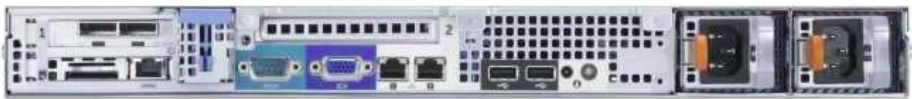
\includegraphics{imatges/ser_back.png}
\end{quote}

\begin{quote}
2 fonts d'alimentació redundants. Fuente de alimentación: 2 fuentes de alimentación intercambiables en caliente de Dell \textbf{Platinum efficiency 350W or 550W power supply}
\end{quote}

\begin{quote}
Dell OpenManage Systems Management OpenManage Essentials
\end{quote}

\begin{quote}
Acustica, sobre 30db. El posarem en una habitació fora de l'oficina i la sala. No sera problema.
\end{quote}

\hypertarget{switch}{%
\chapter{switch}\label{switch}}

\hypertarget{installaciuxf3-de-wifi}{%
\chapter{Instal·lació de wifi}\label{installaciuxf3-de-wifi}}

\hypertarget{requeriments-per-a-la-seua-implantaciuxf3}{%
\section{Requeriments per a la seua implantació}\label{requeriments-per-a-la-seua-implantaciuxf3}}

Uns repetidors de wifi. S'haguera de pensar si realment es vol instal·lar per tindre cobertura per als 92 espectadors, o es pensa que no tots es connectaran, i començar per un sistema bàsic, ampliable a mesura que augmenten les necessitats. I si es posa, donar-li més ús, no sol accés a internet.

\hypertarget{potuxe8ncia-de-la-connexiuxf3-dinternet-per-donar-servei}{%
\subsection{Potència de la connexió d'internet per donar servei}\label{potuxe8ncia-de-la-connexiuxf3-dinternet-per-donar-servei}}

Es requereix que l'amplada de banda de la connexió d'internet puga donar servei almenys a 92 espectadors, que se l'afore del pati de butaques.

S'ha de limitar l'amplada de banda que oferim als espectadors en cas de realitzar la reproducció en línia al mateix temps, açò ho realitzem assegurant l'amplada de banda en la xarxa del circuit d'imatge. En el commutador. Es recomana contractar una connexió d'amplada de banda minima 300Mb.

\hypertarget{localitzaciuxf3-dels-dispositius-de-retransmissiuxf3}{%
\subsection{Localització dels dispositius de retransmissió}\label{localitzaciuxf3-dels-dispositius-de-retransmissiuxf3}}

Hem d'estudiar el número i posicions en la sala perquè la retransmissió siga òptima. En principi si l'antena és bona, en una en l'entrada de la sala d'actes, seria suficient, o en el sostre, damunt l'escenari. Pero en ser una casa vella de parets immenses, segur hi ha problemes, per a tot l'espai. Es poden posar altres no tan potents, no han de donar servei per a tanta gent.

\hypertarget{muntatge-1}{%
\section{Muntatge}\label{muntatge-1}}

Antena, una d'aquestes de \href{https://ui.com/wi-fi}{Unifi}, recomane U6 Professional, pero no sé en les parets tan grans que hi ha en la sala, valdrà un sol per a tot l'espai. Es pot posar un altre repetidor sol per al despatx. La idea és fer dues xarxes, una per al públic, en accés a internet i al servidor web intern de promocions, i una altra que tinga accés a la xarxa de l'oficina i recursos del servidor, que podem utilitzar perquè el centre de llums comunique en el servidor de fitxers, utilitzar camera del movil en espectacles, i xat intern.

Les antenes proposades són PoE, les alimentarem amb el switch, en portar cable de xarxa ja ho tenim.

\href{https://www.ui.com/download/unifi/default/default/unifi-dream-router-datasheet}{Software i documentació}, posar-lo en una VM, en el servidor. \href{https://dl.ui.com/unifi/7.1.61/unifi_sysvinit_all.deb}{Paquet .deb}, per instal.lar en la màquina que fem servir de servidor. min 2GB de Ram, 20 GB hd. \href{https://dl.ui.com/ds/u6-pro_ds}{Especificacions antena pro}

\hypertarget{com-fer-ho}{%
\section{Com fer-ho}\label{com-fer-ho}}

\href{https://www.adamintech.com/ubiquiti-unifi-with-pfsense-and-other-routers/}{unifi wifi en pfsense}

\href{https://lawrence.technology/networking/unifi-pfsense-deployment-setup-and-planning-with-wifi-vlan-guest-network/}{video de la festa}

Els punts d'accés WiFi tenen dos tipus: encaminadors híbrids SOHO on tant l'encaminador com els punts d'accés es combinen en un sol per simplificar l'experiència mitjana d'Internet de la casa. Un altre és simplement un punt d'accés WiFi autònom que funciona per si sol i que depèn d'un encaminador independent per a DHCP/encaminament a Internet. Per a això, estudiarem la configuració d'un punt d'accés WiFi autònom amb Ubiquiti UniFi.

La Ubiquiti UniFi AP-AC Lite admet una velocitat wifi de fins a 300 Mbps a 2,4 GHz i 867 Mbps a una freqüència de 5 GHz. Els productes UniFi d'Ubiquiti utilitzen una cosa anomenada ``controlador de xarxa UniFi'', que és un programari que s'executa al vostre ordinador/servidor per gestionar diversos punts d'accés i configuració/provisionalment. És necessari per al subministrament per primera vegada del nostre punt d'accés UniFi, però no és necessari que s'execute constantment, ja que tota la configuració s'emmagatzema al mateix dispositiu.

Comenceu baixant l'instal·lador des d'aquí \href{https://dl.ui.com/unifi/5.11.46/UniFi-installer.exe}{UniFi-Installer} .per a windows. El controlador de xarxa UniFi depen de Java per funcionar.

\href{https://blog.barclayhowe.com/setting-up-a-vlan-in-pfsense-and-unifi/}{latra milloor vlan wifi}

\hypertarget{unifi-ap-amb-pfsense-vlan}{%
\section{UniFi AP amb pfSense VLAN}\label{unifi-ap-amb-pfsense-vlan}}

\href{https://brendonmatheson.com/2020/03/14/unifi-ap-with-pfsense-vlans.html}{altra, una privada i altra publica, soles internet}

\hypertarget{infraestructura-1}{%
\subsection{Infraestructura}\label{infraestructura-1}}

\begin{itemize}
\tightlist
\item
  Tallafoc/encaminador pfSense construït en un mini-PC sense ventilador amb una CPU Core i5, 8 GB de RAM i 6 NIC en 2 sobra, una per a l'entrada amb l'encaminador i l'altra per a l'eixida.
\item
  UniFi Controller que s'executa en un Raspberry Pi (part del meu projecte de node de control)
\item
  Punt d'accés UniFi nano HD
\end{itemize}

Passa del switch per fer les VLAN

\hypertarget{procediment}{%
\subsection{Procediment}\label{procediment}}

\begin{itemize}
\tightlist
\item
  Definiu les VLAN i les subxarxes a pfSense
\item
  Configureu DHCP a pfSense
\item
  Configureu les regles del tallafoc a pfSense
\item
  Mapar les VLAN al controlador UniFi
\item
  Definiu els SSID WiFi al controlador UniFi
\end{itemize}

Definir les xarxes wifi

\begin{itemize}
\tightlist
\item
  Privada
\item
  Pública
\item
  Video, No internet
\end{itemize}

La diferència entre aquests és que la xarxa privada (Verda) pot accedir als recursos de la xarxa interna, Nextcloud, registrador de video \ldots{}

\hypertarget{definiu-les-vlan-i-les-subxarxes-a-pfsense}{%
\subsection{Definiu les VLAN i les subxarxes a pfSense}\label{definiu-les-vlan-i-les-subxarxes-a-pfsense}}

\begin{itemize}
\tightlist
\item
  Sense etiquetar - ``VERD'' - per a ordinadors i serveis de confiança a la LAN per cable.
\item
  20 - ``Privada'' - per a dispositius WiFi de confiança, com ara els nostres telèfons i ordinadors portàtils.
\item
  30 - ``Pública'' - per a dispositius WiFi no fiables i com ara telèfons i ordinadors portàtils dels convidats.
\end{itemize}

Ja tinc el segon port de l'encaminador (igb1) configurat com a VERD amb la subxarxa 192.168.56.0/24.

\hypertarget{per-crear-les-vlan}{%
\subsubsection{Per crear les VLAN:}\label{per-crear-les-vlan}}

\begin{itemize}
\tightlist
\item
  Aneu a Interfícies \textgreater{} Tasques
\item
  Feu clic a la pestanya VLAN
\item
  Feu clic al botó Afegeix per definir la primera VLAN que serà Privada
\item
  Seleccioneu la interfície principal perquè siga igb1: la interfície on es troba la xarxa Verda LAN.
\item
  Introduïu l'etiqueta ``20''
\item
  Introduïu la descripció Privada
\item
  Desa
\end{itemize}

Repetim els mateixos passos per a la pública i la de video amb 30 i 40 com a VLAN.

Les tres aniran per la mateixa interface, la LAN em1, \emph{mirar de crear tres virtuals, ja que totes estan dins el mateix server, no boba totes ha d'eixir cap a l'encaminador}

Més tard afegirem la configuració al commutador perquè puga mapar les VLAN a l'AP, però de moment hem de definir les xarxes per a aquestes VLAN:

\hypertarget{definir-xarxes}{%
\subsubsection{Definir xarxes}\label{definir-xarxes}}

\begin{itemize}
\tightlist
\item
  Feu clic a la pestanya Assignacions de la interfície
\item
  A la fila inferior de la taula, seleccioneu la primera VLAN ``VLAN 20 a igb1 - opt2 (Privat)'' i feu clic a Afegeix
\item
  Feu clic al nom de la interfície predeterminat que es va generar per a aquesta interfície per obrir-ne la configuració
\item
  Marqueu Habilita la interfície
\item
  Canvieu la descripció a ``Privat'' per a més claredat
\item
  A Configuració IPv4 estàtica, introduïu l'adreça de la passarel·la per a aquesta interfície i especifiqueu la mida de la subxarxa. Per a la meua xarxa Privat, li vaig donar la passarel·la 192.168.56.1 amb la subxarxa /24. (Li donem la ip 1 de la xarxa a la interfade del pfsense d'aquesta xarxa)
\end{itemize}

El mateix per a les altres dues xarxes

\hypertarget{configureu-dhcp-a-pfsense}{%
\subsubsection{Configureu DHCP a pfSense}\label{configureu-dhcp-a-pfsense}}

Ara configurem el servei DHCP per a aquestes tres xarxes VLAN noves:

\begin{itemize}
\tightlist
\item
  Seleccioneu Serveis \textgreater{} Servidor DHCP
\item
  Seleccioneu la pestanya Privat
\item
  Marqueu Habilita DHCP
\item
  Introduïu l'interval DHCP: en el meu cas, vaig triar de 192.168.56.100 a 192.168.56.254.
\item
  Desa
\end{itemize}

Repetir el mateix per a les altres dues. Amb xarxa 192.168.80.0/24 per a xarxa pública i 192.168.56.100/24 per a la de video.

L'antena wifi té capacitat per a 300 connexions, l'aforament de públic és de 92, igual haguérem de restringir a 150 la màscara de xarxa, la de video en principi serien és per si es vol connectar algun movil a la xarxa perquè faça de webcam a l'espectacle, l'enregistrador de video, i si es vol connectar la taula de llums, equip de reproducció en continu o edició. La privada els serveis, treballadors, VPN, per wifi, no seran molts, una 15 com a molt. Entre video i personal no crec que siguen més de 20 en el millor cas, pero tampoc vull limitar les connexions públiques per si es fa un altre acte amb més aforament. Si es podria reservar una 20 per si de cas amb la màscara de xarxa de la pública.

\hypertarget{configura-les-regles-del-tallafoc-a-pfsense}{%
\subsubsection{Configura les regles del tallafoc a pfSense}\label{configura-les-regles-del-tallafoc-a-pfsense}}

Estableix les regles com s'adrecen per permetre l'entrada o la sortida del trànsit. La diferència clau entre Pública i privat és que privat pot accedir a interna i internet, pública soles a internat, i Video no tindrà accés a internet.

Això s'aconsegueix definint primer un àlies anomenat rfc1918\_networks que agrupa els blocs CIDR per als dominis no encaminables Firewall -\textgreater{} aliases -\textgreater{} edit

\begin{figure}
\centering
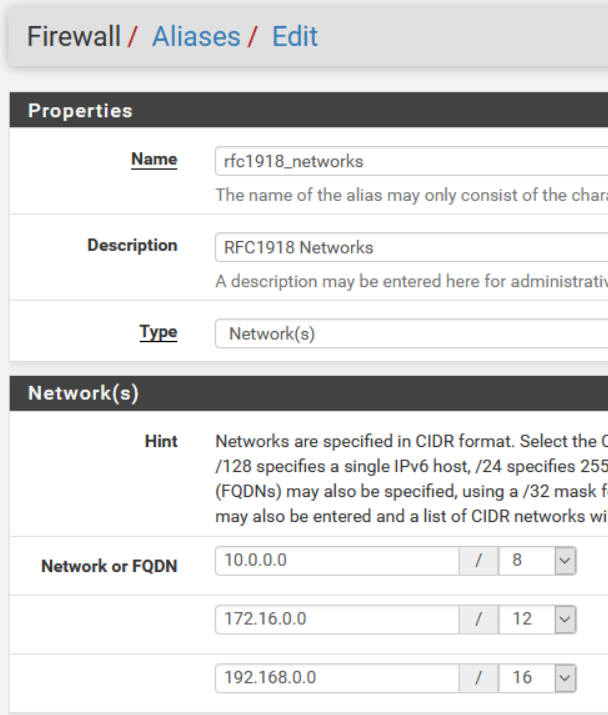
\includegraphics{imatges/pfsense_aliase_prov.png}
\caption{aliases providsional}
\end{figure}

A continuació, definim una regla per permetre les destinacions que no es troben en aquest rang (tingueu en compte el doble negatiu) mentre que la regla de catchall final bloqueja l'accés

\begin{figure}
\centering
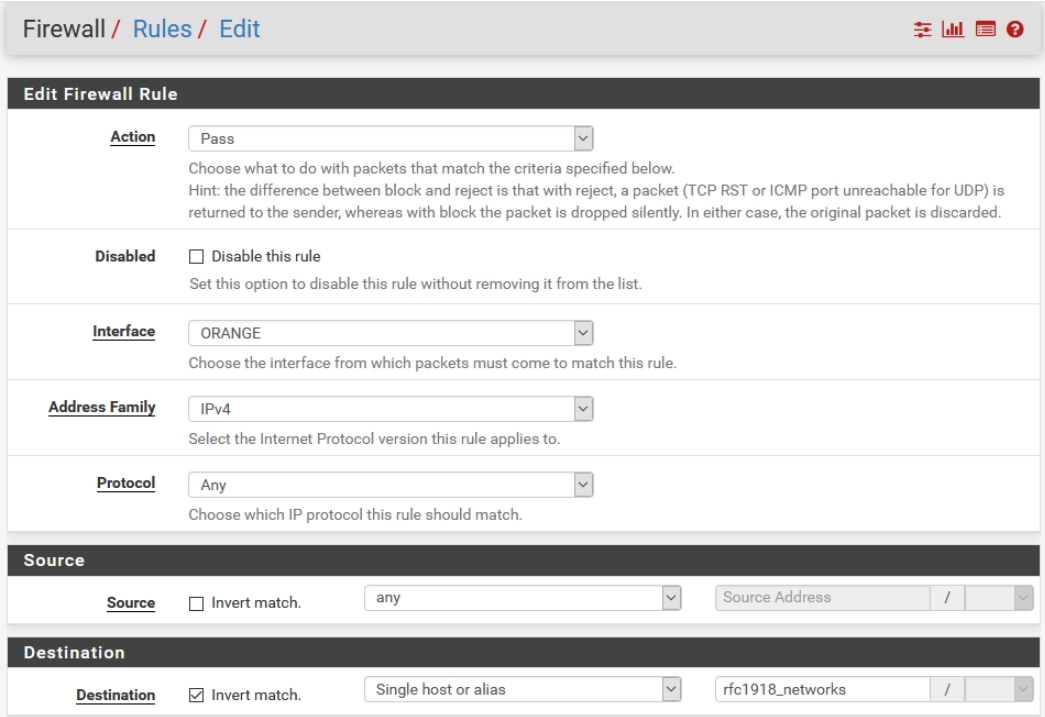
\includegraphics{imatges/regles prov.png}
\caption{regles prov}
\end{figure}

Això permet explícitament que Pública accedisca a Internet (adreces que no són rfc1918) mentre que la regla de catchall bloqueja l'accés a adreces locals a Pública.

\textbf{Falta mirar video no vaja a internat, supose sera en action no pass}

\hypertarget{assigna-les-vlan-al-controlador-unifi}{%
\subsection{Assigna les VLAN al controlador UniFi}\label{assigna-les-vlan-al-controlador-unifi}}

A continuació, anem a UniFi Controller per assignar les VLAN als SSID WiFi

\begin{itemize}
\tightlist
\item
  A la configuració, feu clic a Xarxes i després a Crea una xarxa nova.
\item
  Seleccioneu VLAN Només per al propòsit, poseu un nom a la xarxa Privat i doneu-li l'etiqueta VLAN 20 com vam fer a pfSense
\end{itemize}

\begin{figure}
\centering
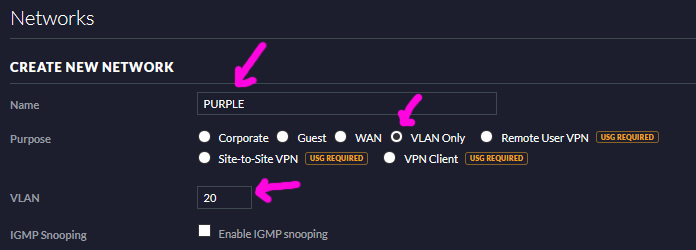
\includegraphics{imatges/wifi/unifi_01_purple_vlan.png}
\caption{crea wifi privat}
\end{figure}

\begin{itemize}
\tightlist
\item
  Deseu la xarxa i feu el mateix per definir la VLAN Pública
\item
  Després de desar aquestes dues xarxes, es mostraran a la llista de xarxes; confirmeu que són correctes
\end{itemize}

\begin{figure}
\centering
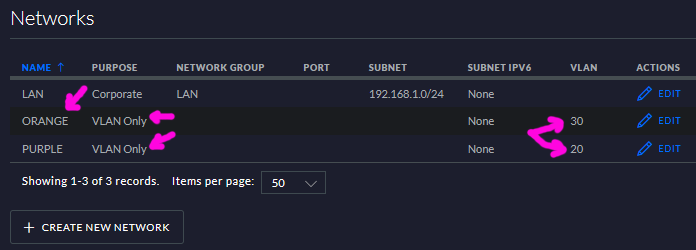
\includegraphics{imatges/wifi/unifi_03_vlans.png}
\caption{xarxes wifi}
\end{figure}

\hypertarget{definiu-els-ssid-de-wifi-a-unifi-controller}{%
\subsubsection{Definiu els SSID de WiFi a UniFi Controller}\label{definiu-els-ssid-de-wifi-a-unifi-controller}}

A continuació, crearem els SSID de WiFi i els enllaçarem a les nostres VLAN

\begin{itemize}
\tightlist
\item
  Al menú Configuració, trieu Xarxes sense fil (just a sobre de Xarxes) i feu clic a Crea una xarxa sense fil nova
\item
  Doneu el nom SSID ``Privat'' i configureu el xifratge com corresponga (p.~ex. WPA-PSK)
\item
  Feu clic a Opcions avançades per mostrar el camp de l'etiqueta VLAN i introduïu 20 perquè aquest SSID gestionarà el trànsit de la VLAN Privat.
\end{itemize}

\begin{figure}
\centering
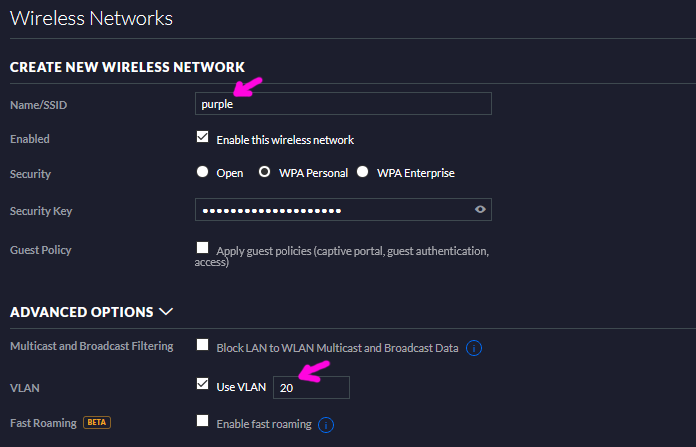
\includegraphics{imatges/wifi/unifi_04_privat_ssid.png}
\caption{xarxa privat ssdi}
\end{figure}

La publica i video, de la mateixa forma.

\hypertarget{unifi-pfsense}{%
\subsection{unifi-pfsense}\label{unifi-pfsense}}

Un script que instal·la el programari UniFi Controller a pfSense i altres sistemes FreeBSD \href{https://github.com/unofficial-unifi/unifi-pfsense}{repositori}

Perill, es trenca si pfSense està en MBR Aquest script destruirà un sistema BIOS heretat arrencat des d'un volum arrel ZFS amb format MBR Per evitar aquest problema, utilitzeu el mode UEFI si està disponible, feu servir particions GPT o utilitzeu un sistema de fitxers diferent de ZFS.

L'actualitzador de pfSense eliminarà tot el que instal·leu que no haja arribat a pfSense, inclosos els paquets instal·lats per aquest script.

Després d'actualitzar pfSense, haureu de tornar a executar aquest script per restaurar les dependències i el programari.

Massa pegues.

\hypertarget{rack}{%
\chapter{Rack}\label{rack}}

  \bibliography{book.bib,packages.bib}

\end{document}
